\section*{Mutation and haplotype summary}

\begin{figure*}[h]
    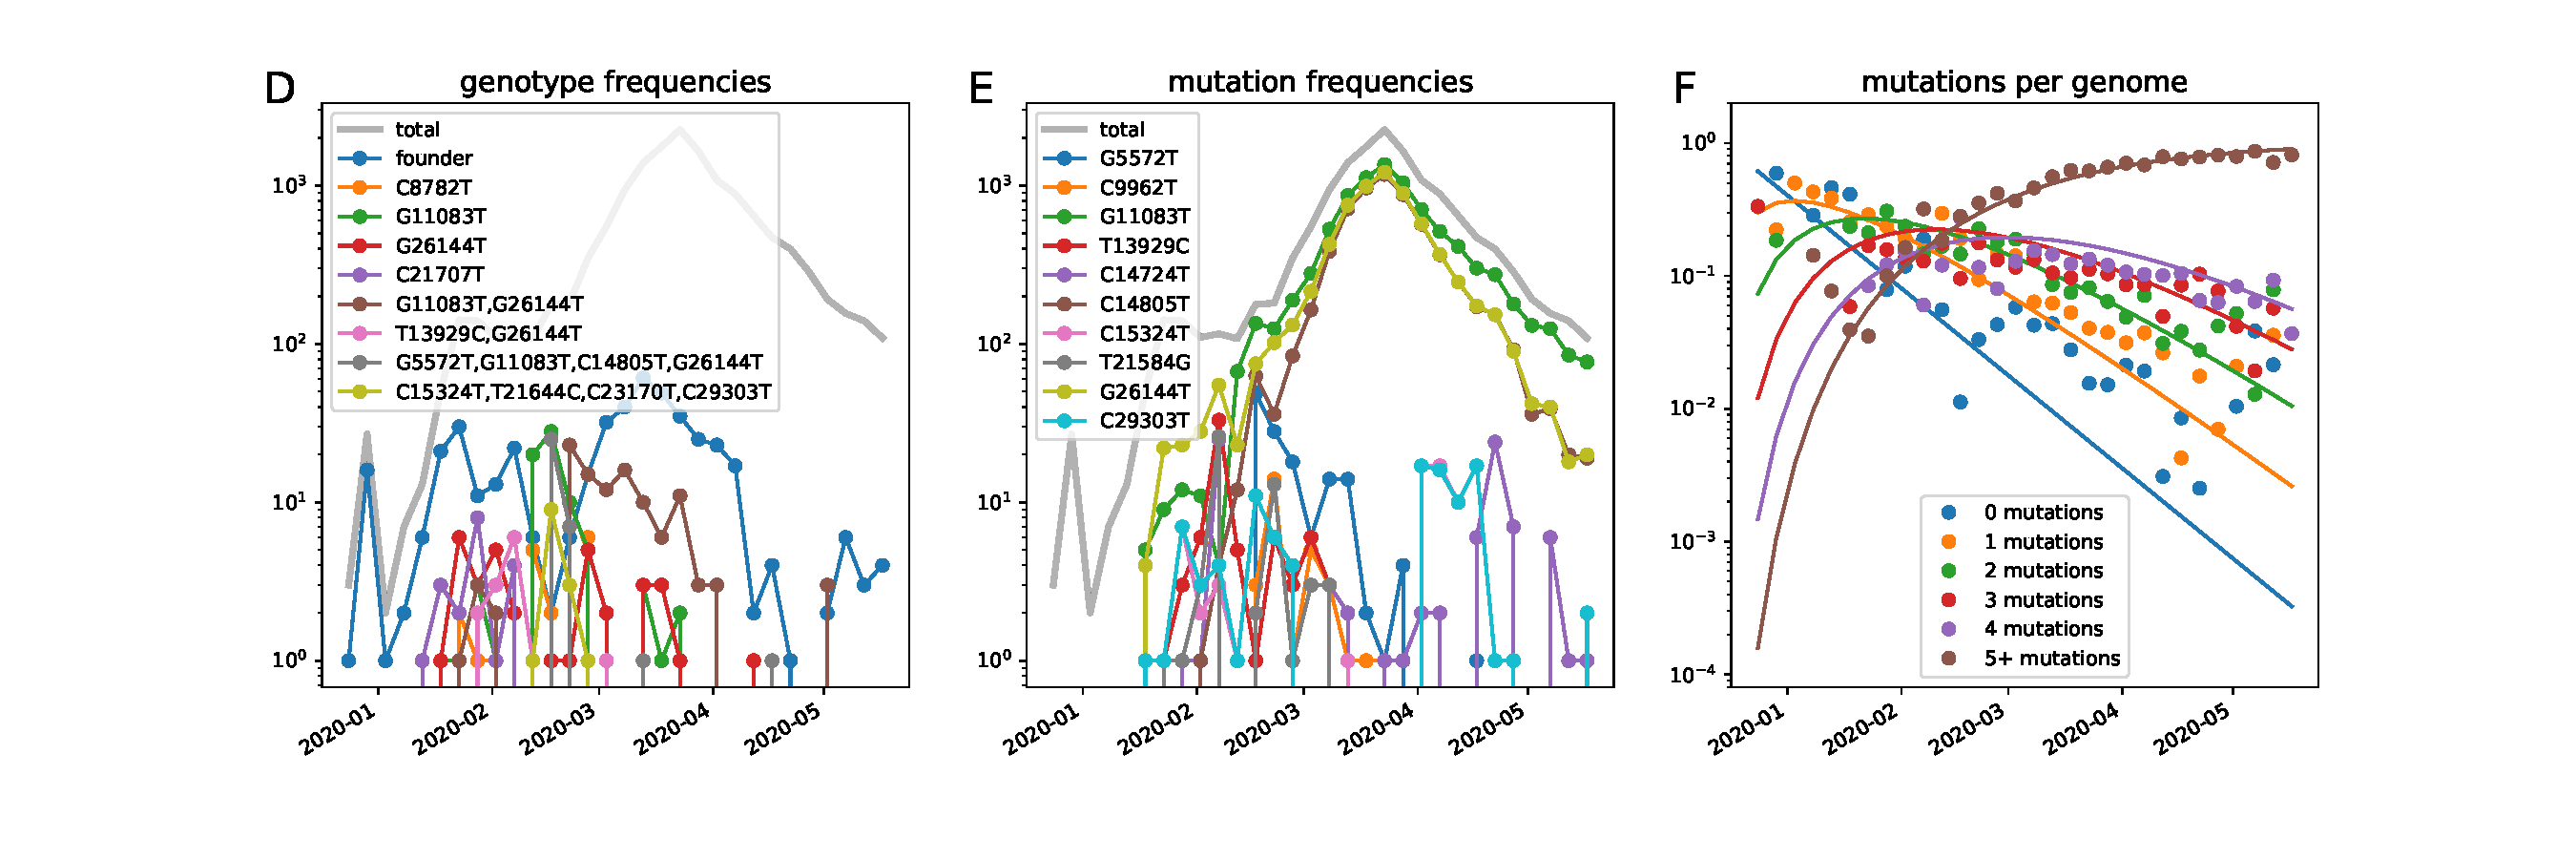
\includegraphics[width=\textwidth]{figures/counts/19A_counts.pdf}
    \caption{{\bf Diversification within clade 19A.}
    \label{fig:19A_counts}}
\end{figure*}

\begin{figure*}[h]
    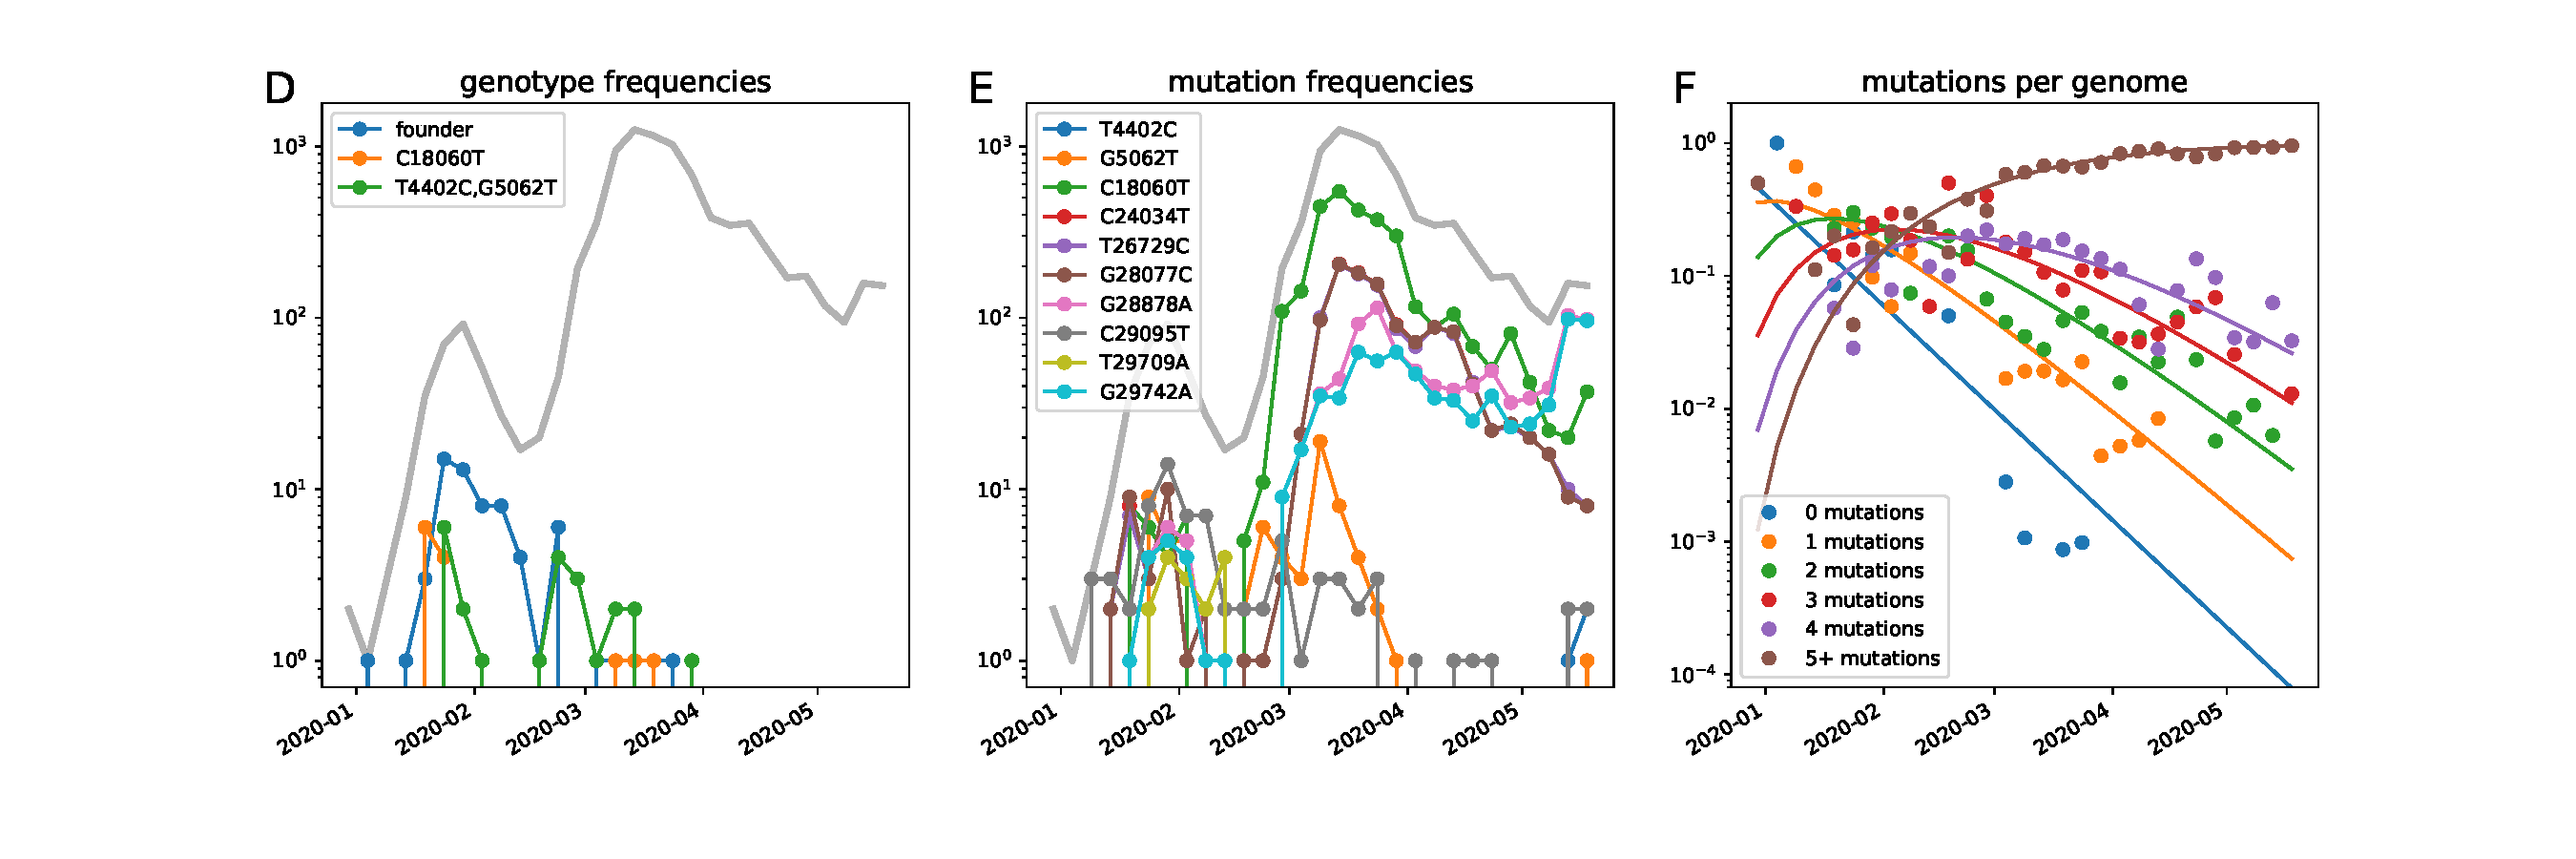
\includegraphics[width=\textwidth]{figures/counts/19B_counts.pdf}
    \caption{{\bf Diversification within clade 19B.}
    \label{fig:19B_counts}}
\end{figure*}

\begin{figure*}[h]
    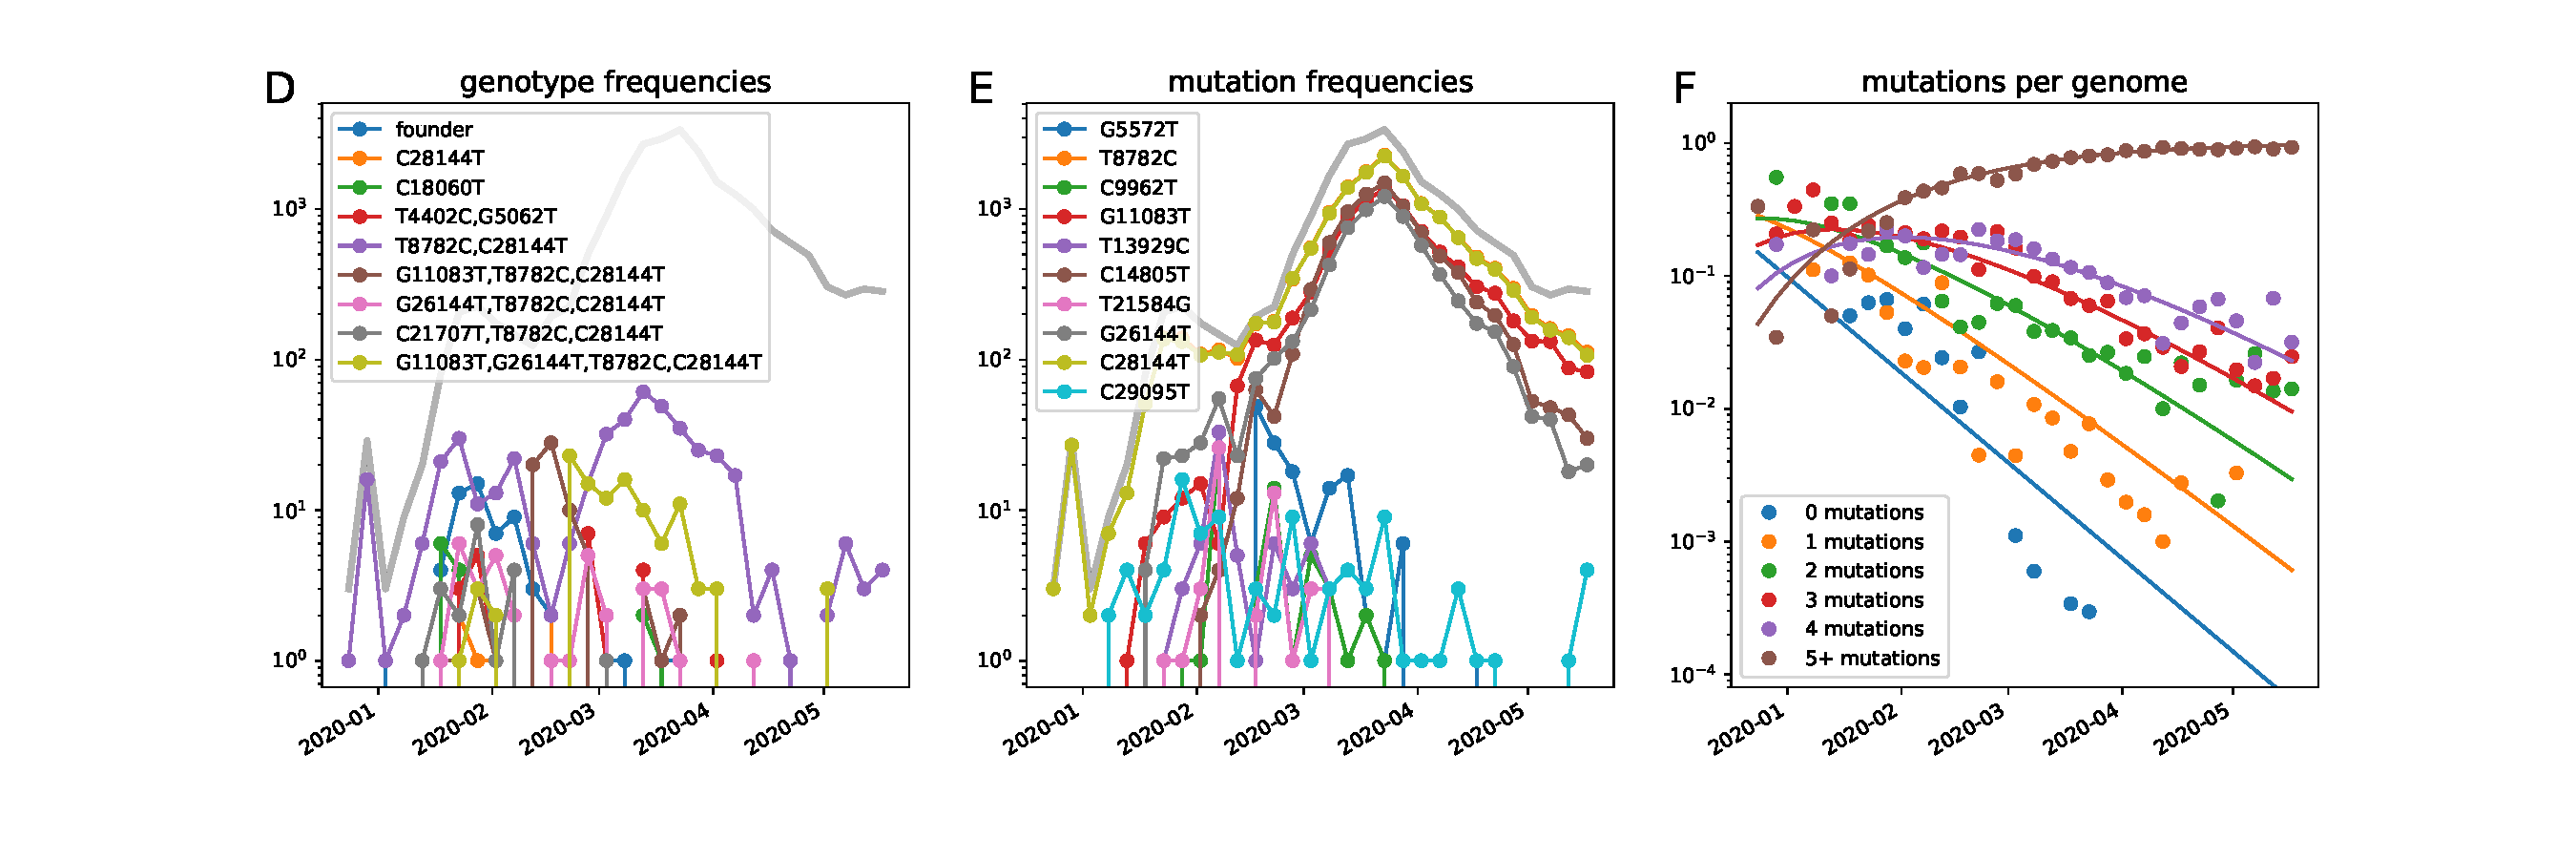
\includegraphics[width=\textwidth]{figures/counts/19B+_counts.pdf}
    \caption{{\bf Diversification within clade 19B+.}
    This figure contains sequences in clades 19 A and B rooted on clade 19B.
    \label{fig:19B+_counts}}
\end{figure*}

\begin{figure*}[h]
    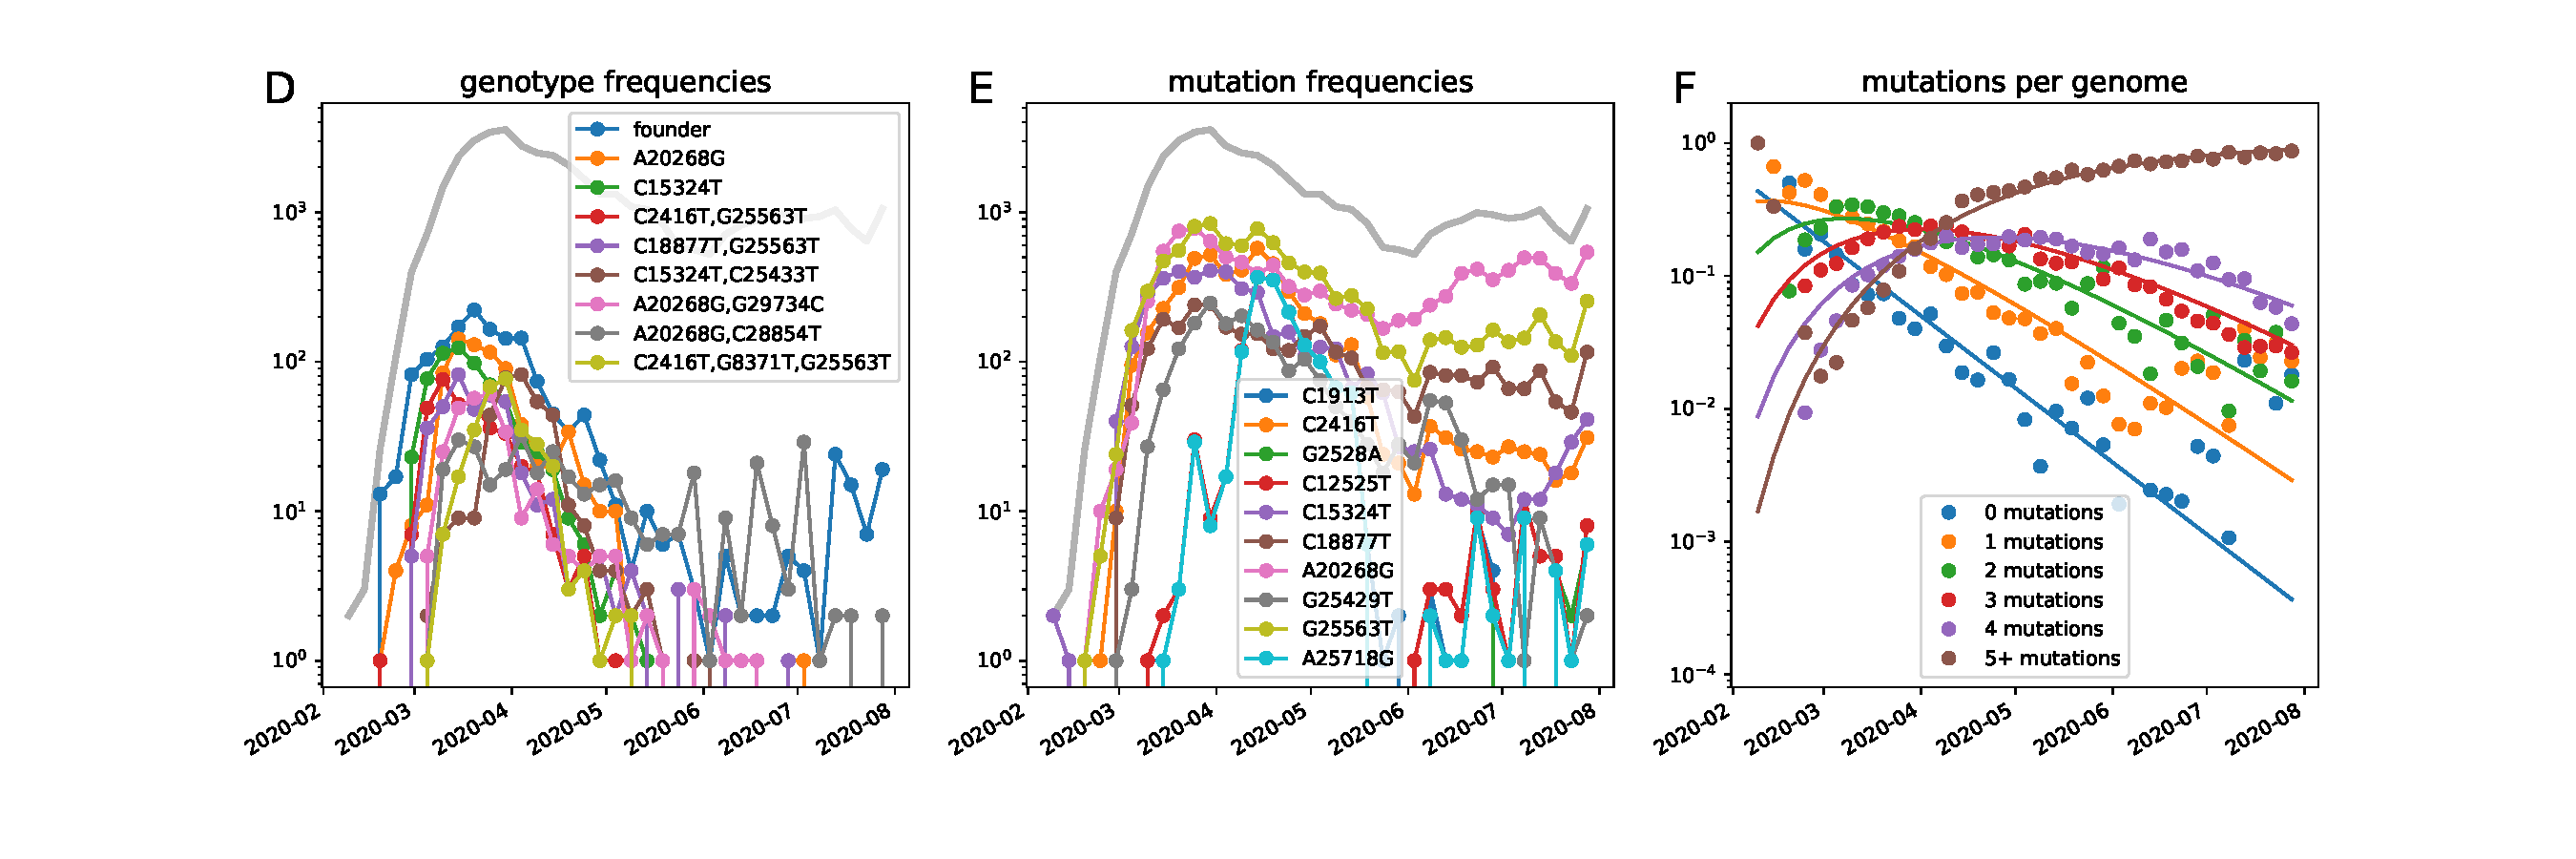
\includegraphics[width=\textwidth]{figures/counts/20A_counts.pdf}
    \caption{{\bf Diversification within clade 20A.}
    \label{fig:20A_counts}}
\end{figure*}

\begin{figure*}[h]
    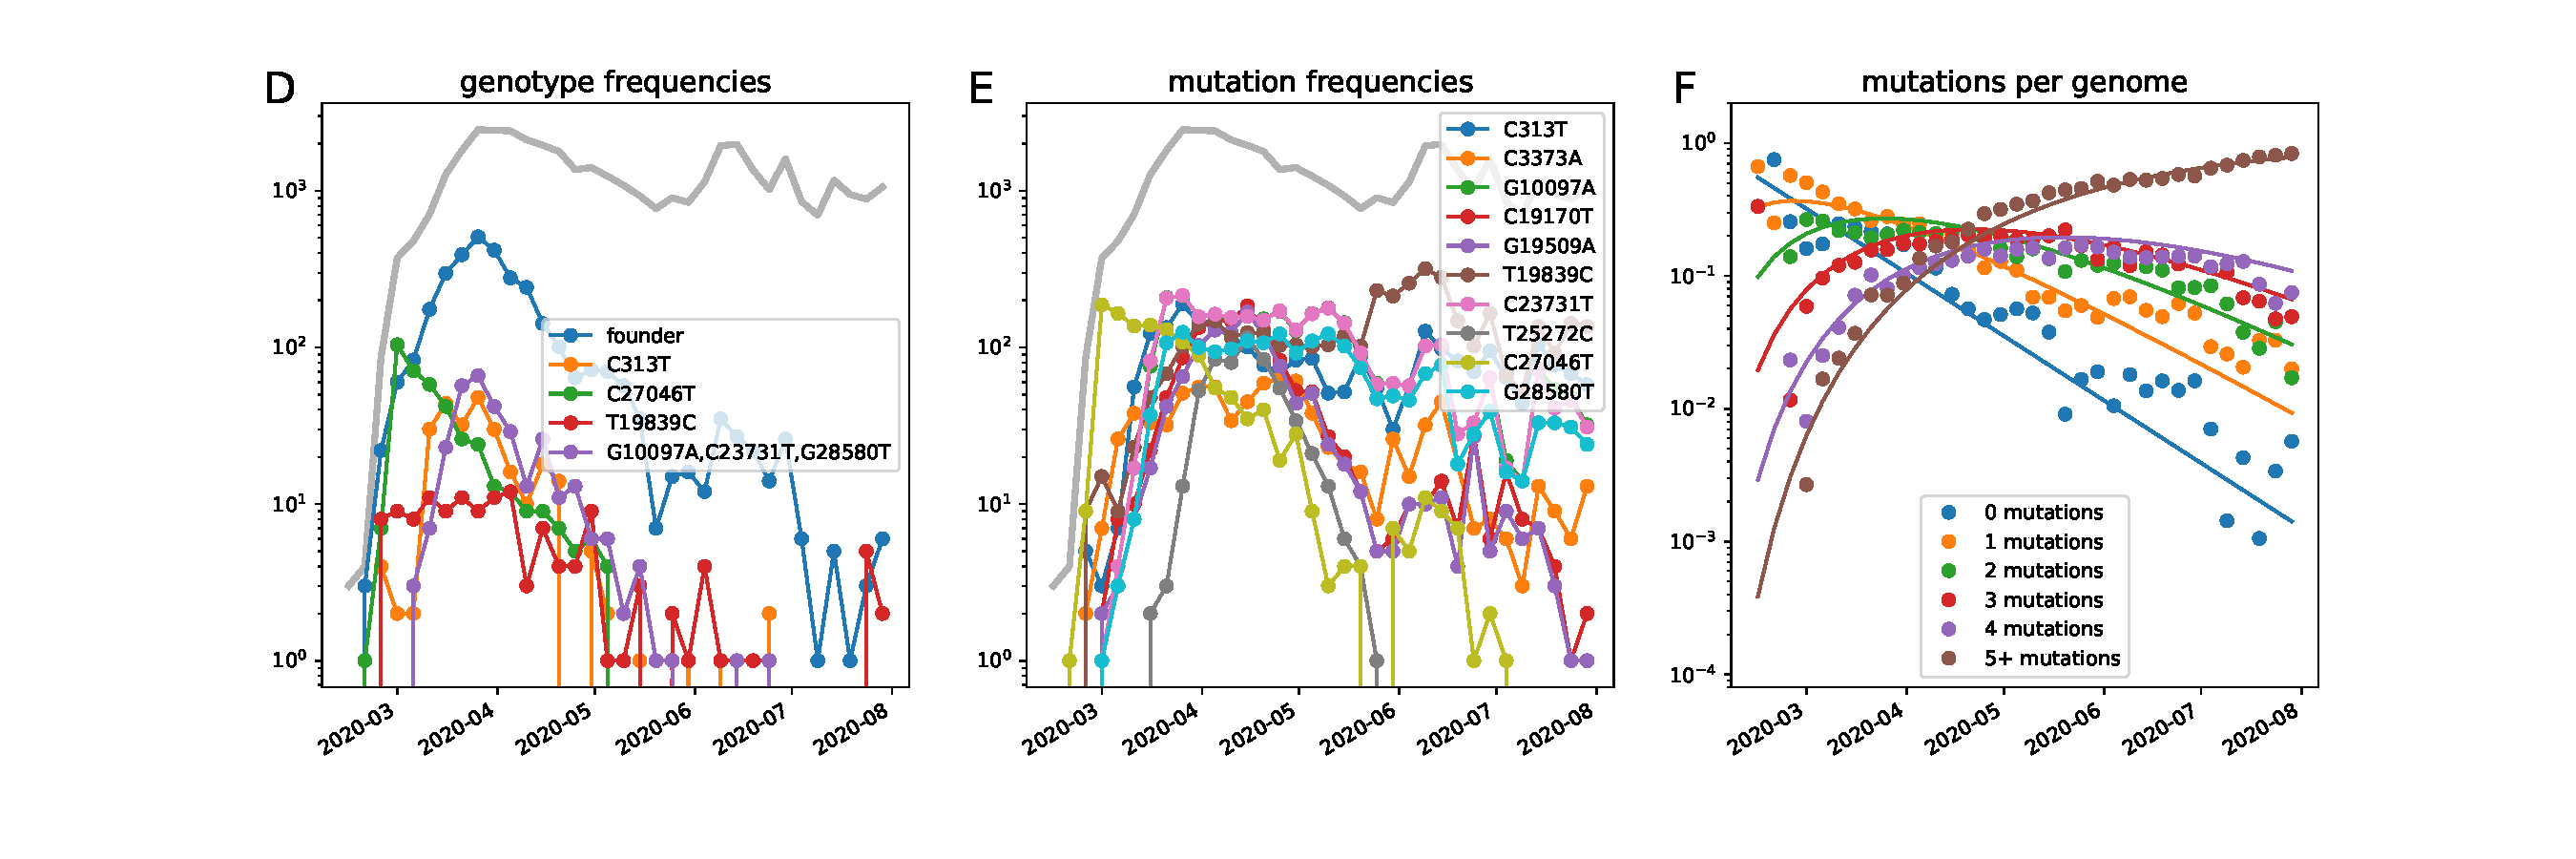
\includegraphics[width=\textwidth]{figures/counts/20B_counts.pdf}
    \caption{{\bf Diversification within clade 20B.}
    \label{fig:20B_counts}}
\end{figure*}

\begin{figure*}[h]
    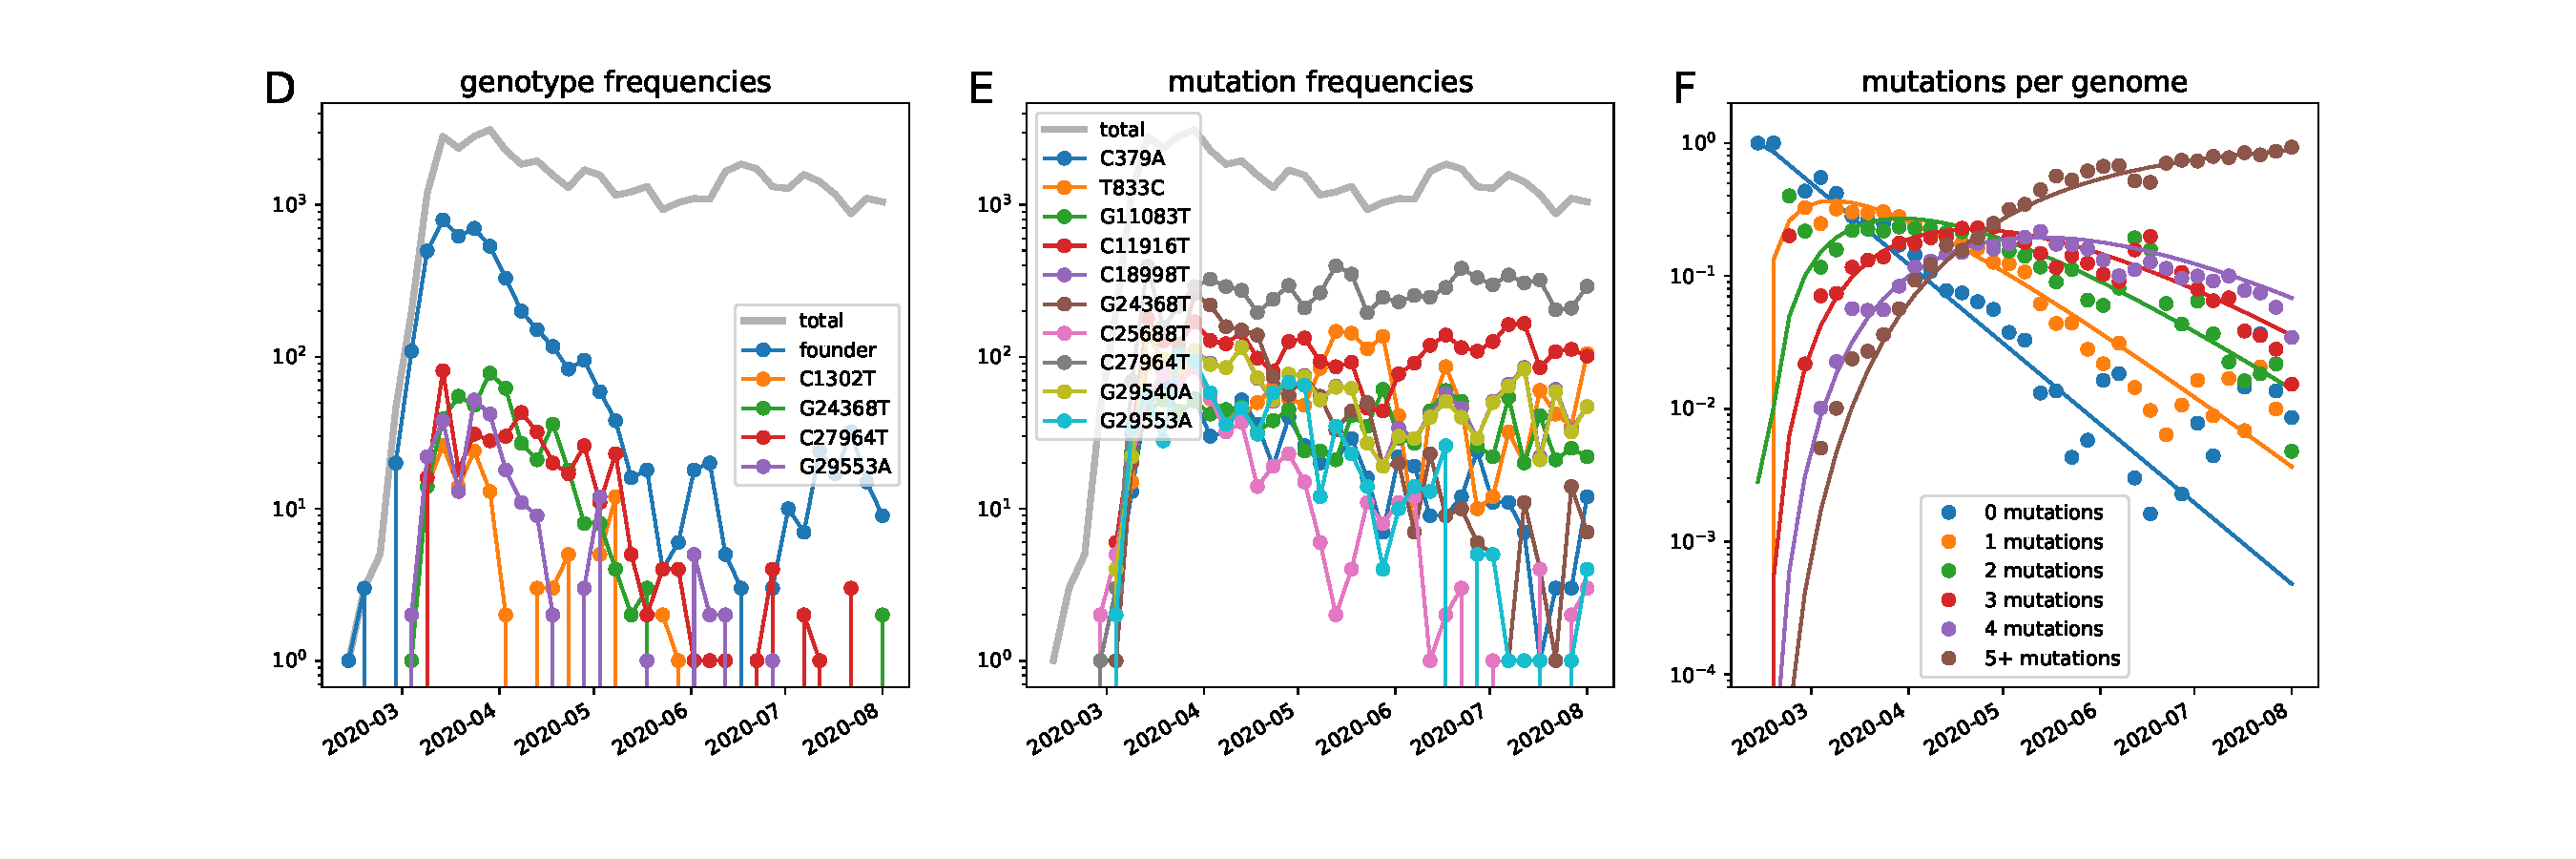
\includegraphics[width=\textwidth]{figures/counts/20C_counts.pdf}
    \caption{{\bf Diversification within clade 20C.}
    \label{fig:20C_counts}}
\end{figure*}


\begin{figure*}[h]
    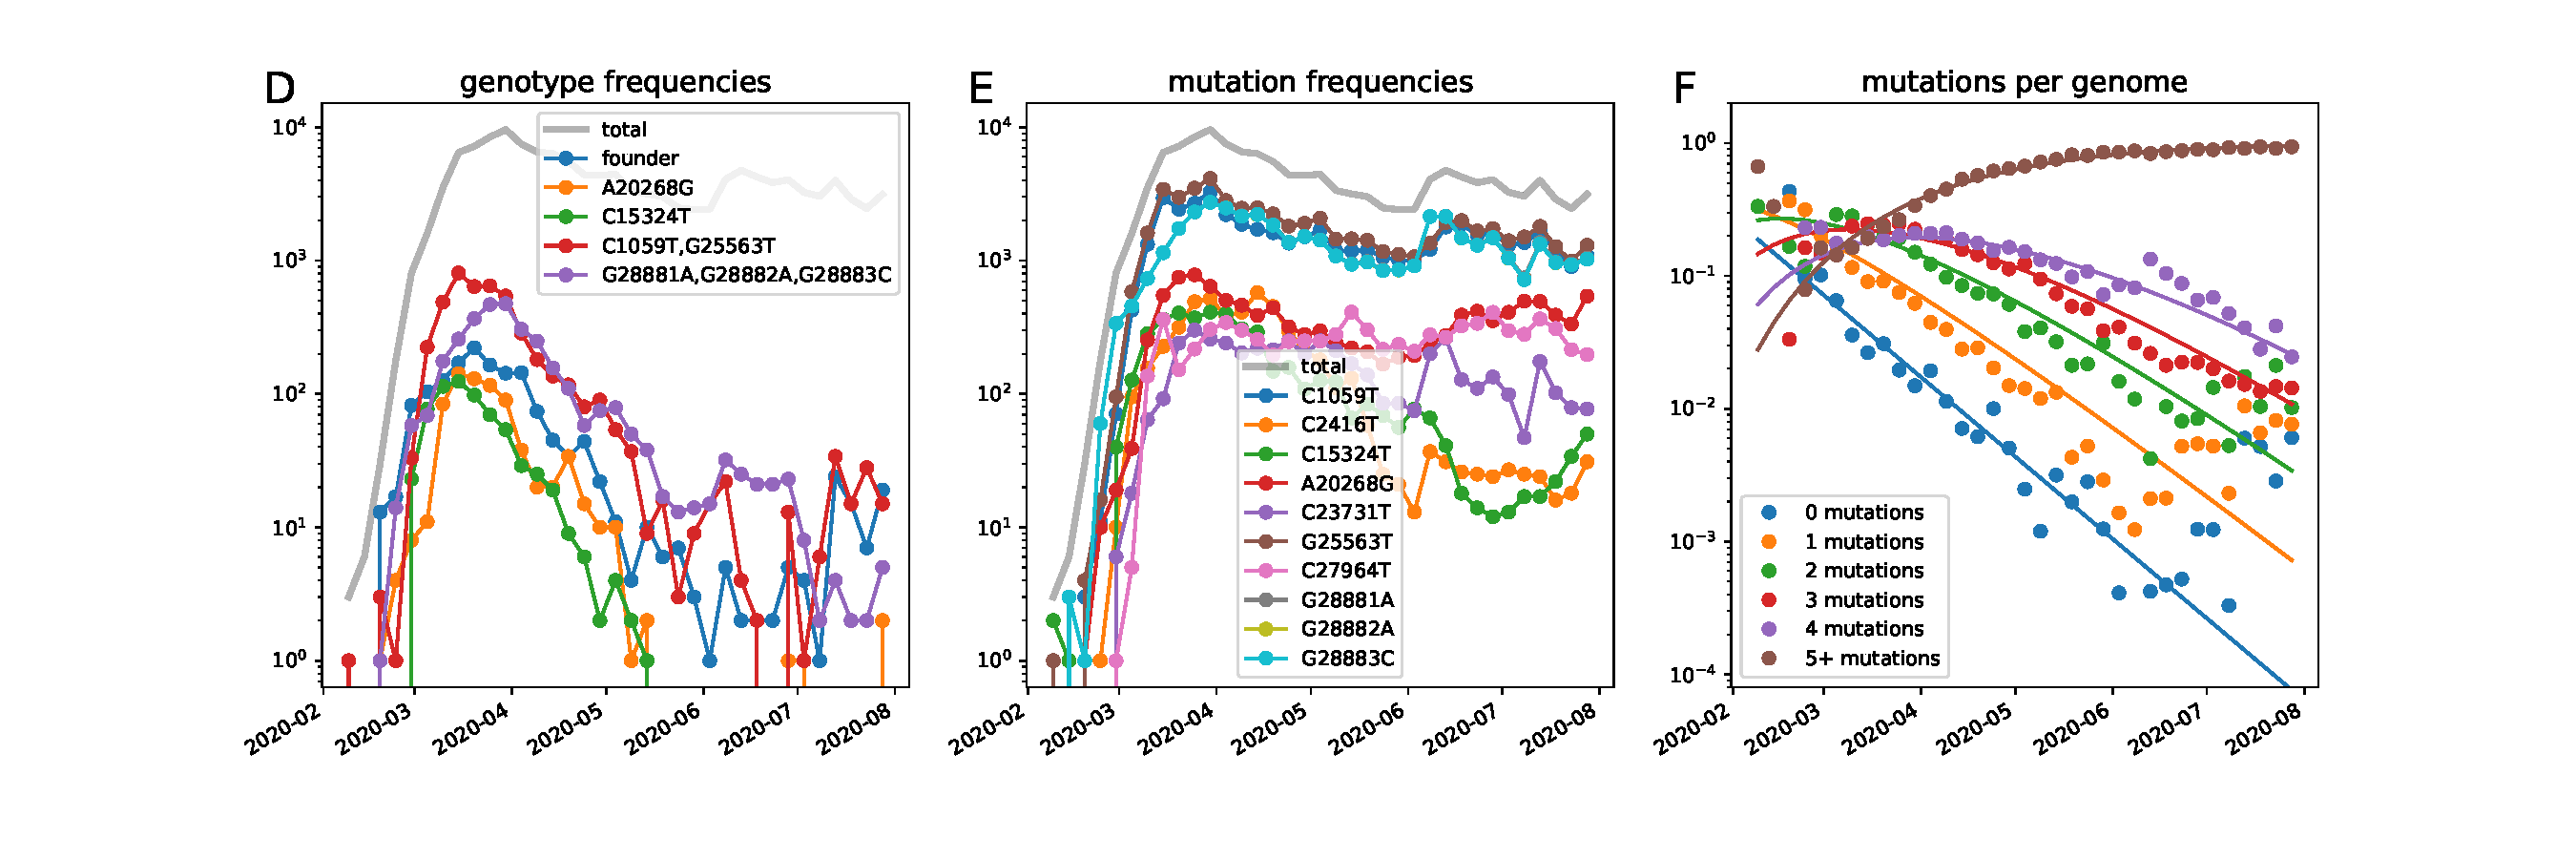
\includegraphics[width=\textwidth]{figures/counts/20A+_counts.pdf}
    \caption{{\bf Diversification within clade 20A+.}
    This figure contains sequences in clades 20A,B,C,D rooted on clade 20A.
    \label{fig:20A+_counts}}
\end{figure*}



\begin{figure*}[h]
    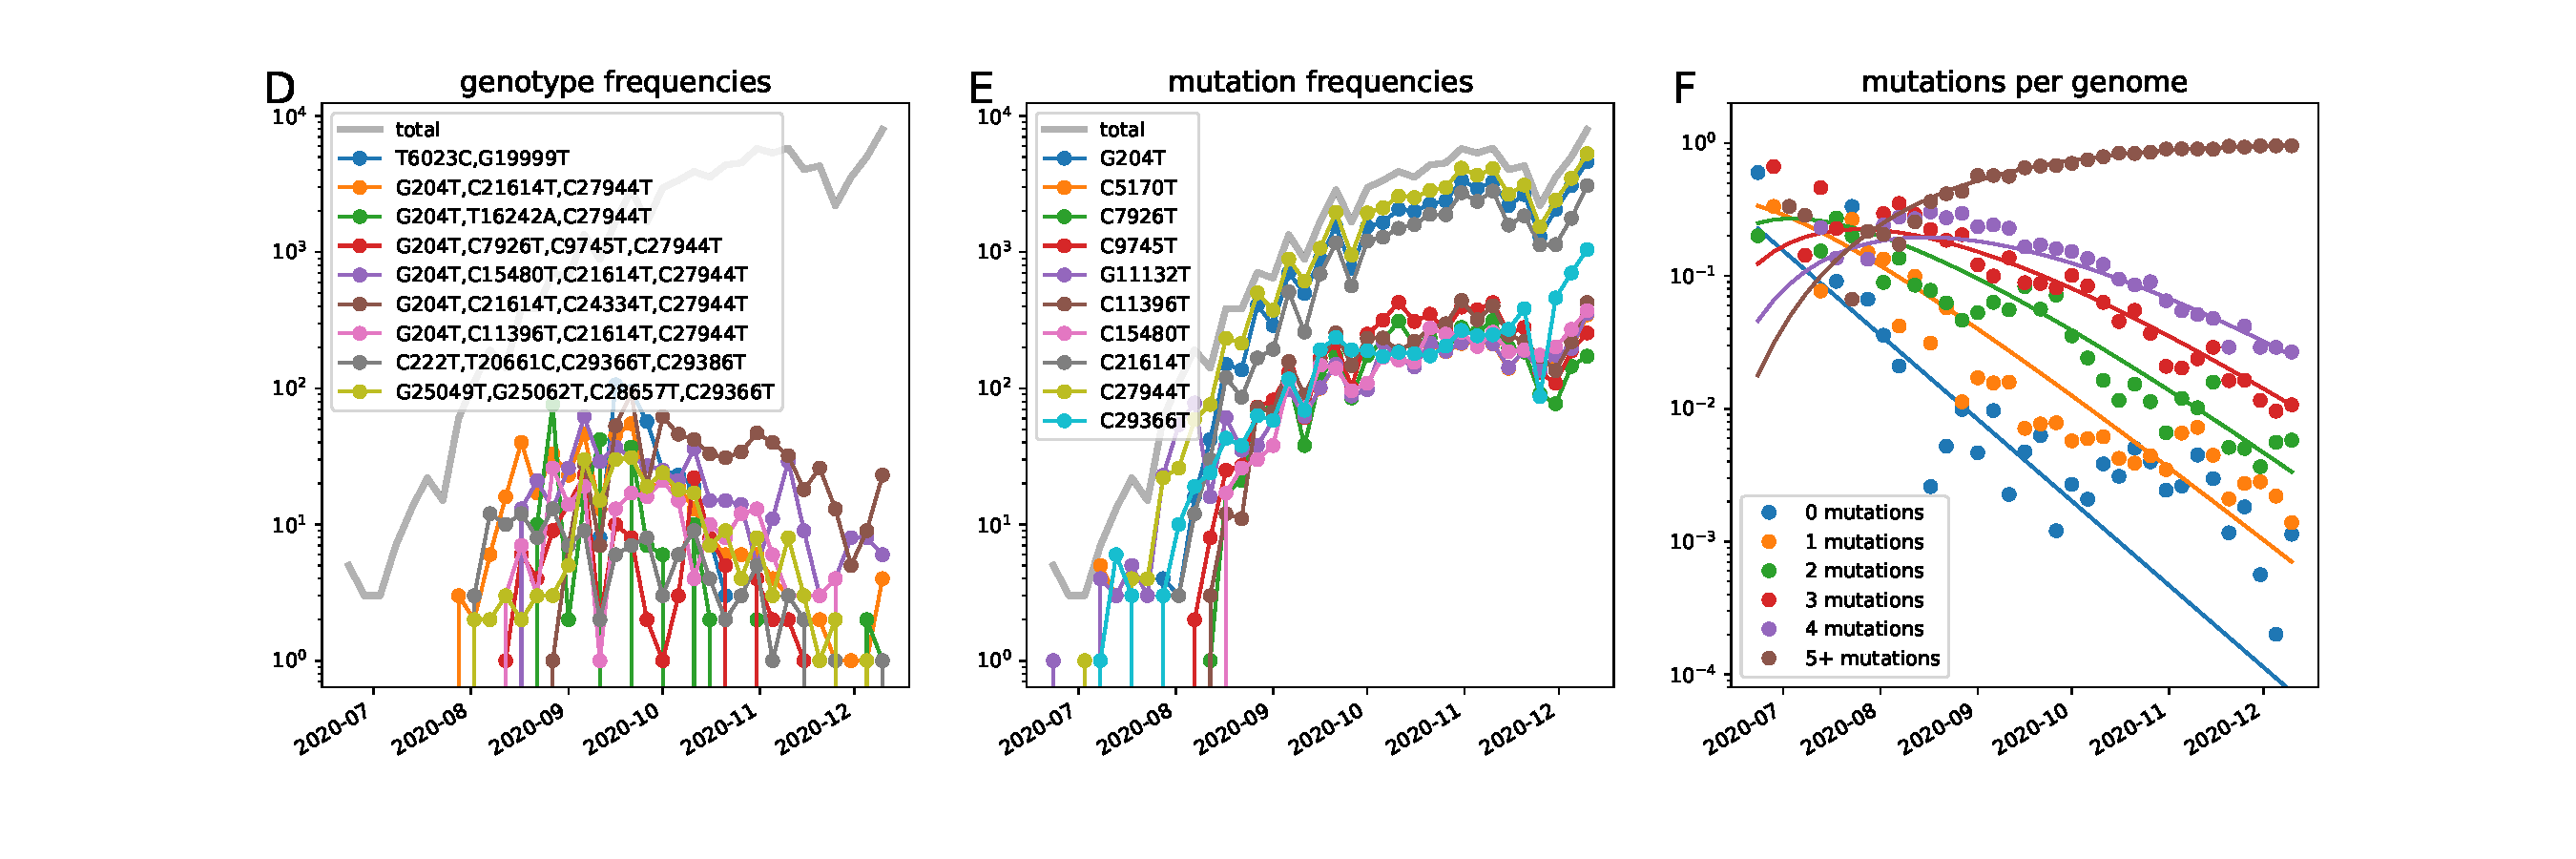
\includegraphics[width=\textwidth]{figures/counts/20E_counts.pdf}
    \caption{{\bf Diversification within clade 20E.}
    \label{fig:20E_counts}}
\end{figure*}

\begin{figure*}[h]
    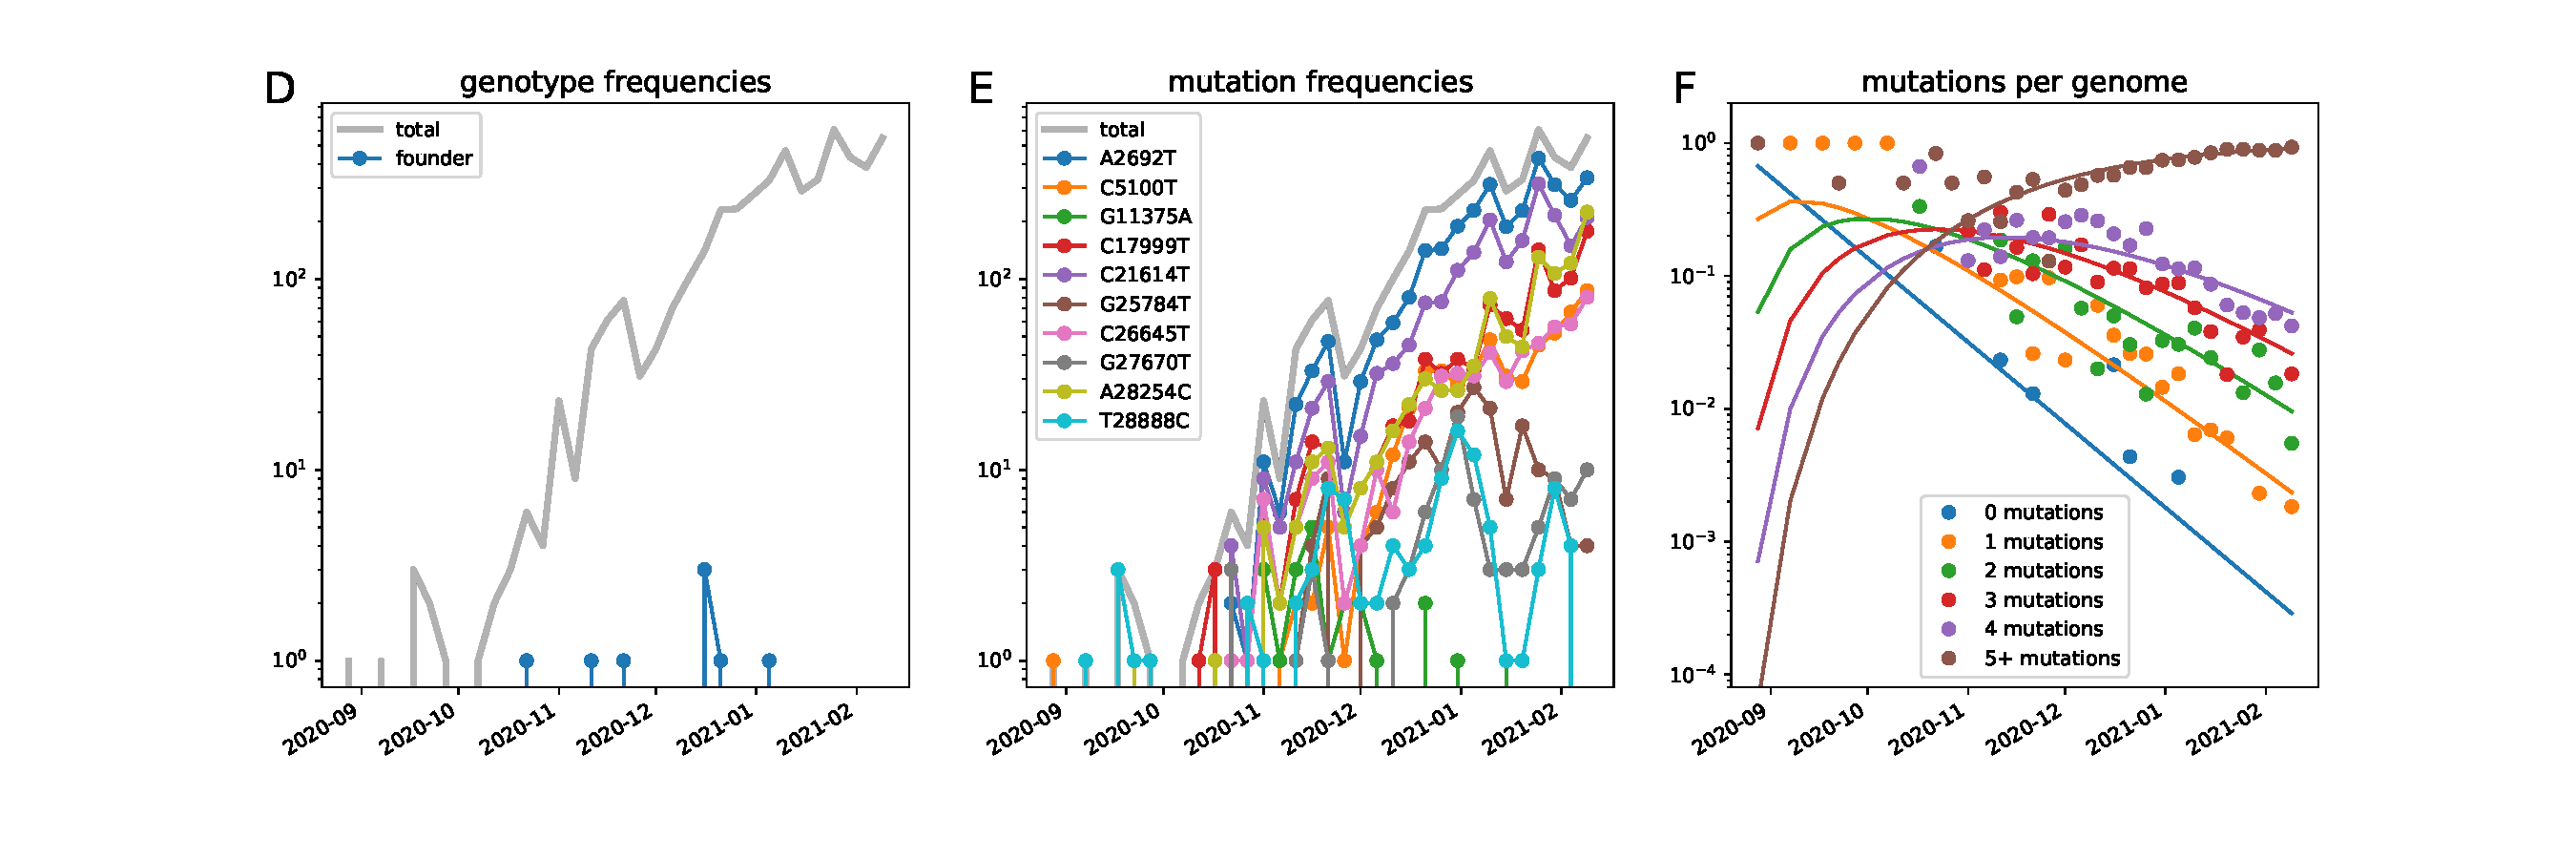
\includegraphics[width=\textwidth]{figures/counts/20H_counts.pdf}
    \caption{{\bf Diversification within clade 20H (Beta).}
    \label{fig:20H_counts}}
\end{figure*}

\begin{figure*}[h]
    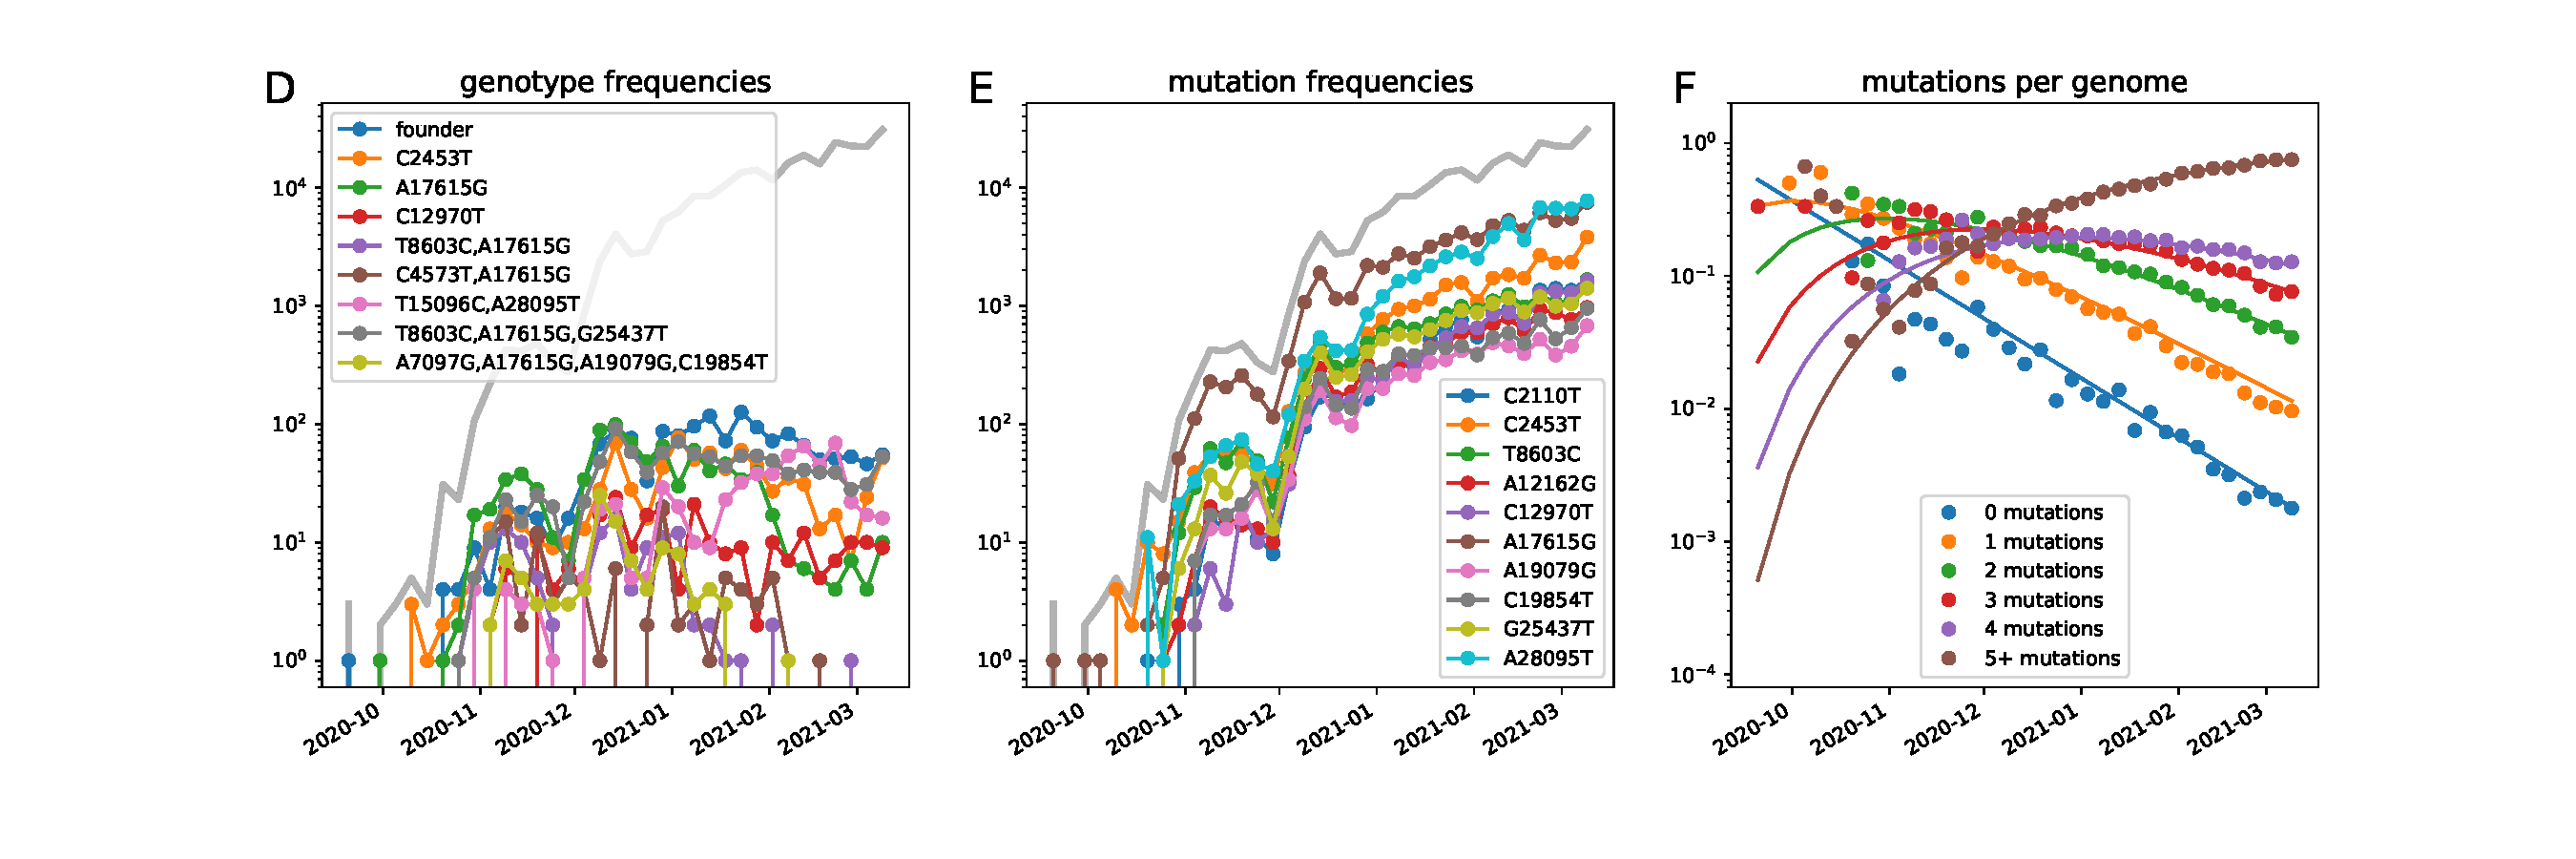
\includegraphics[width=\textwidth]{figures/counts/20I_counts.pdf}
    \caption{{\bf Diversification within clade 20I (Alpha).}
    \label{fig:20I_counts}}
\end{figure*}

\begin{figure*}[h]
    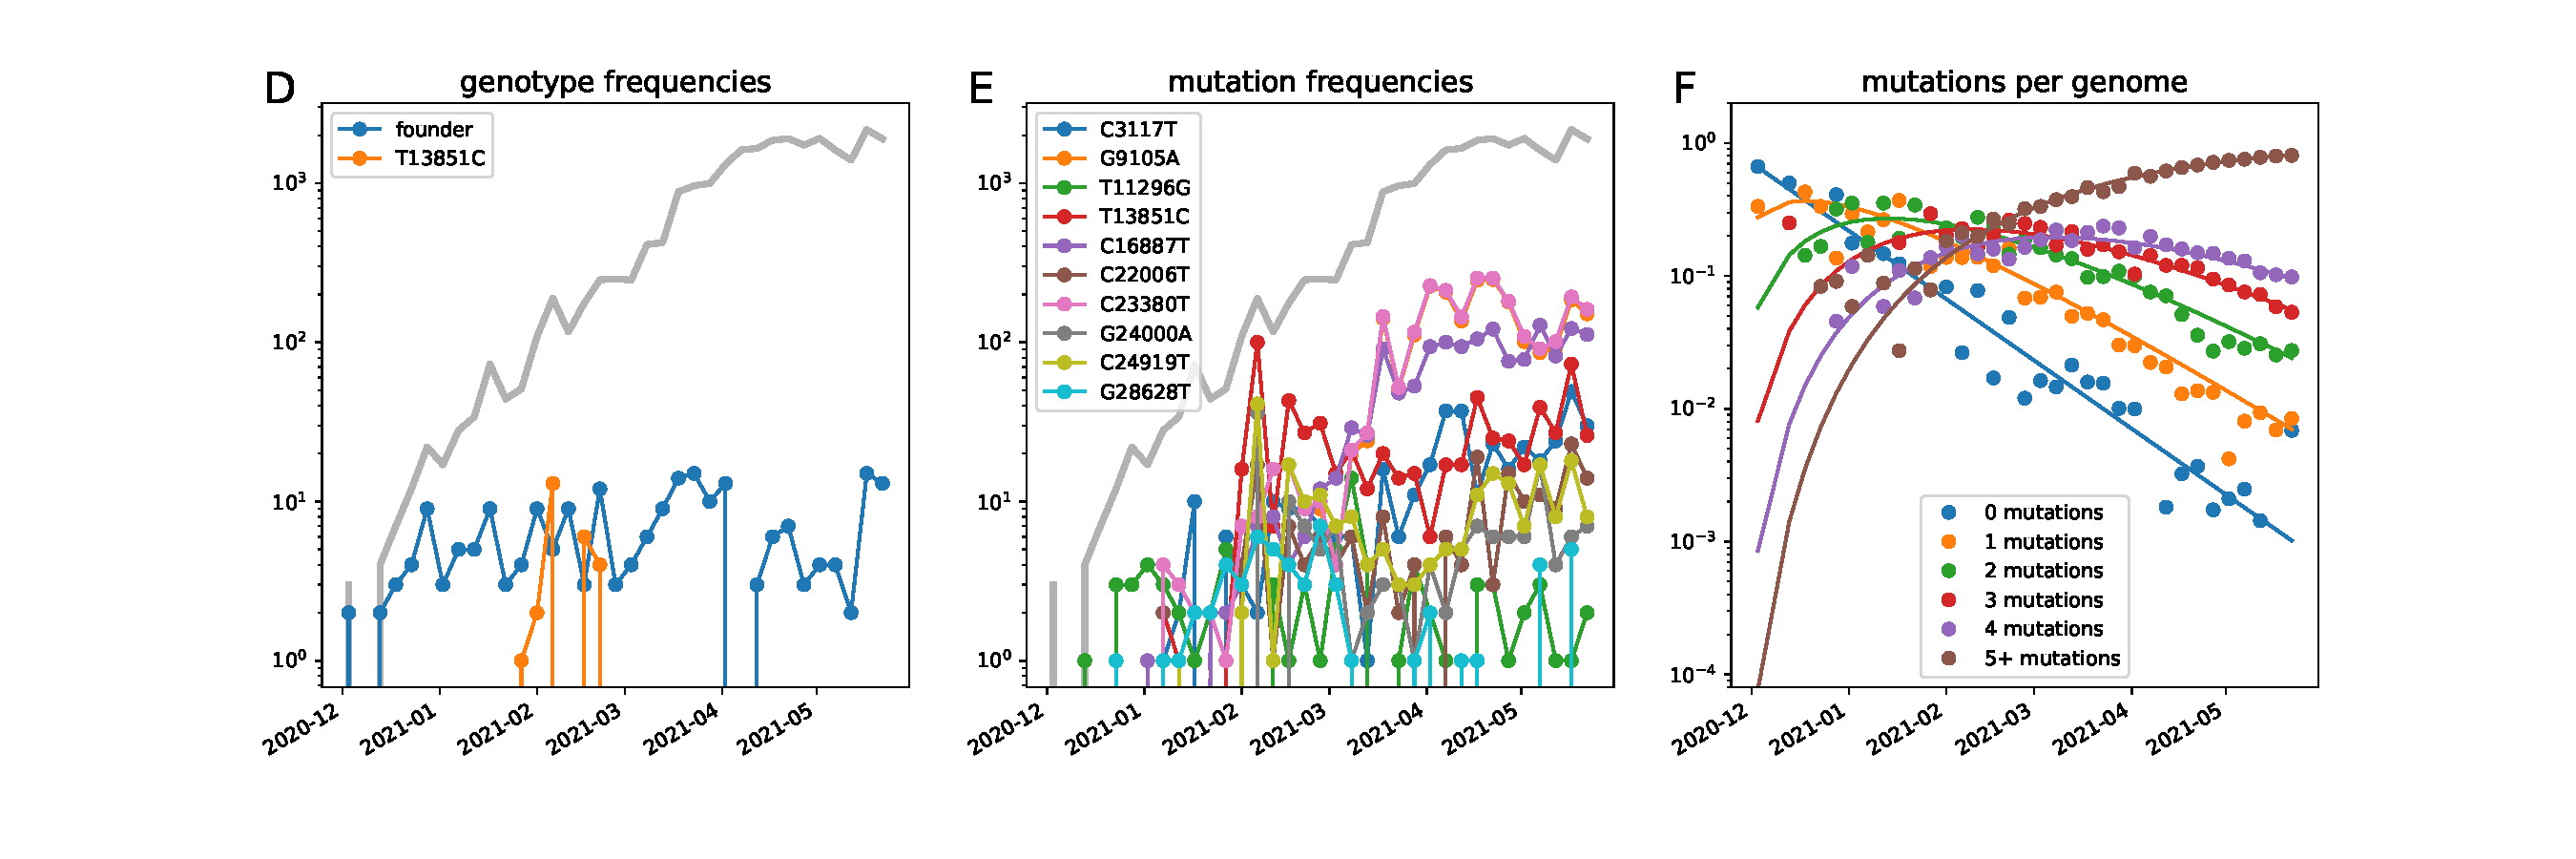
\includegraphics[width=\textwidth]{figures/counts/20J_counts.pdf}
    \caption{{\bf Diversification within clade 20J (Gamma).}
    \label{fig:20J_counts}}
\end{figure*}


\begin{figure*}[h]
    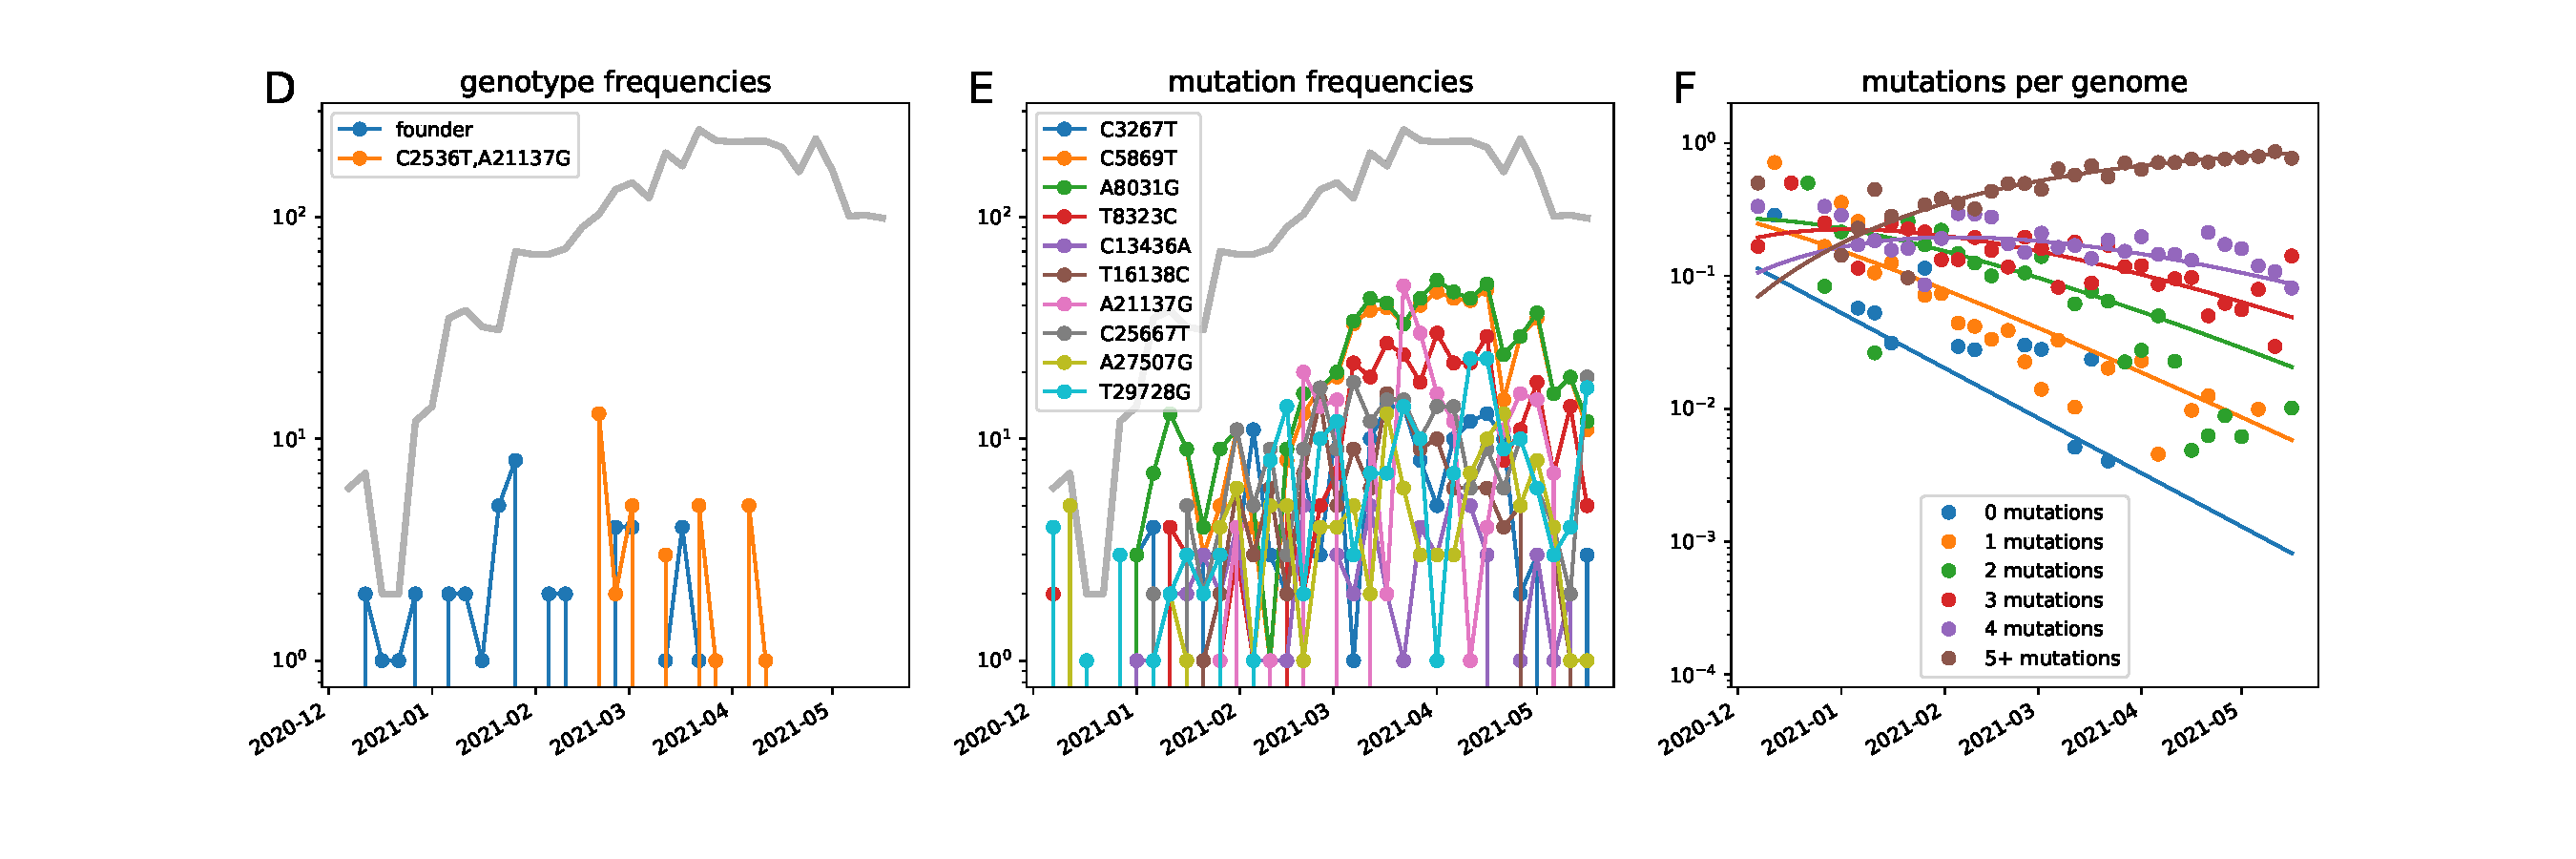
\includegraphics[width=\textwidth]{figures/counts/21D_counts.pdf}
    \caption{{\bf Diversification within clade 21D (Eta).}
    \label{fig:21D_counts}}
\end{figure*}


\begin{figure*}[h]
    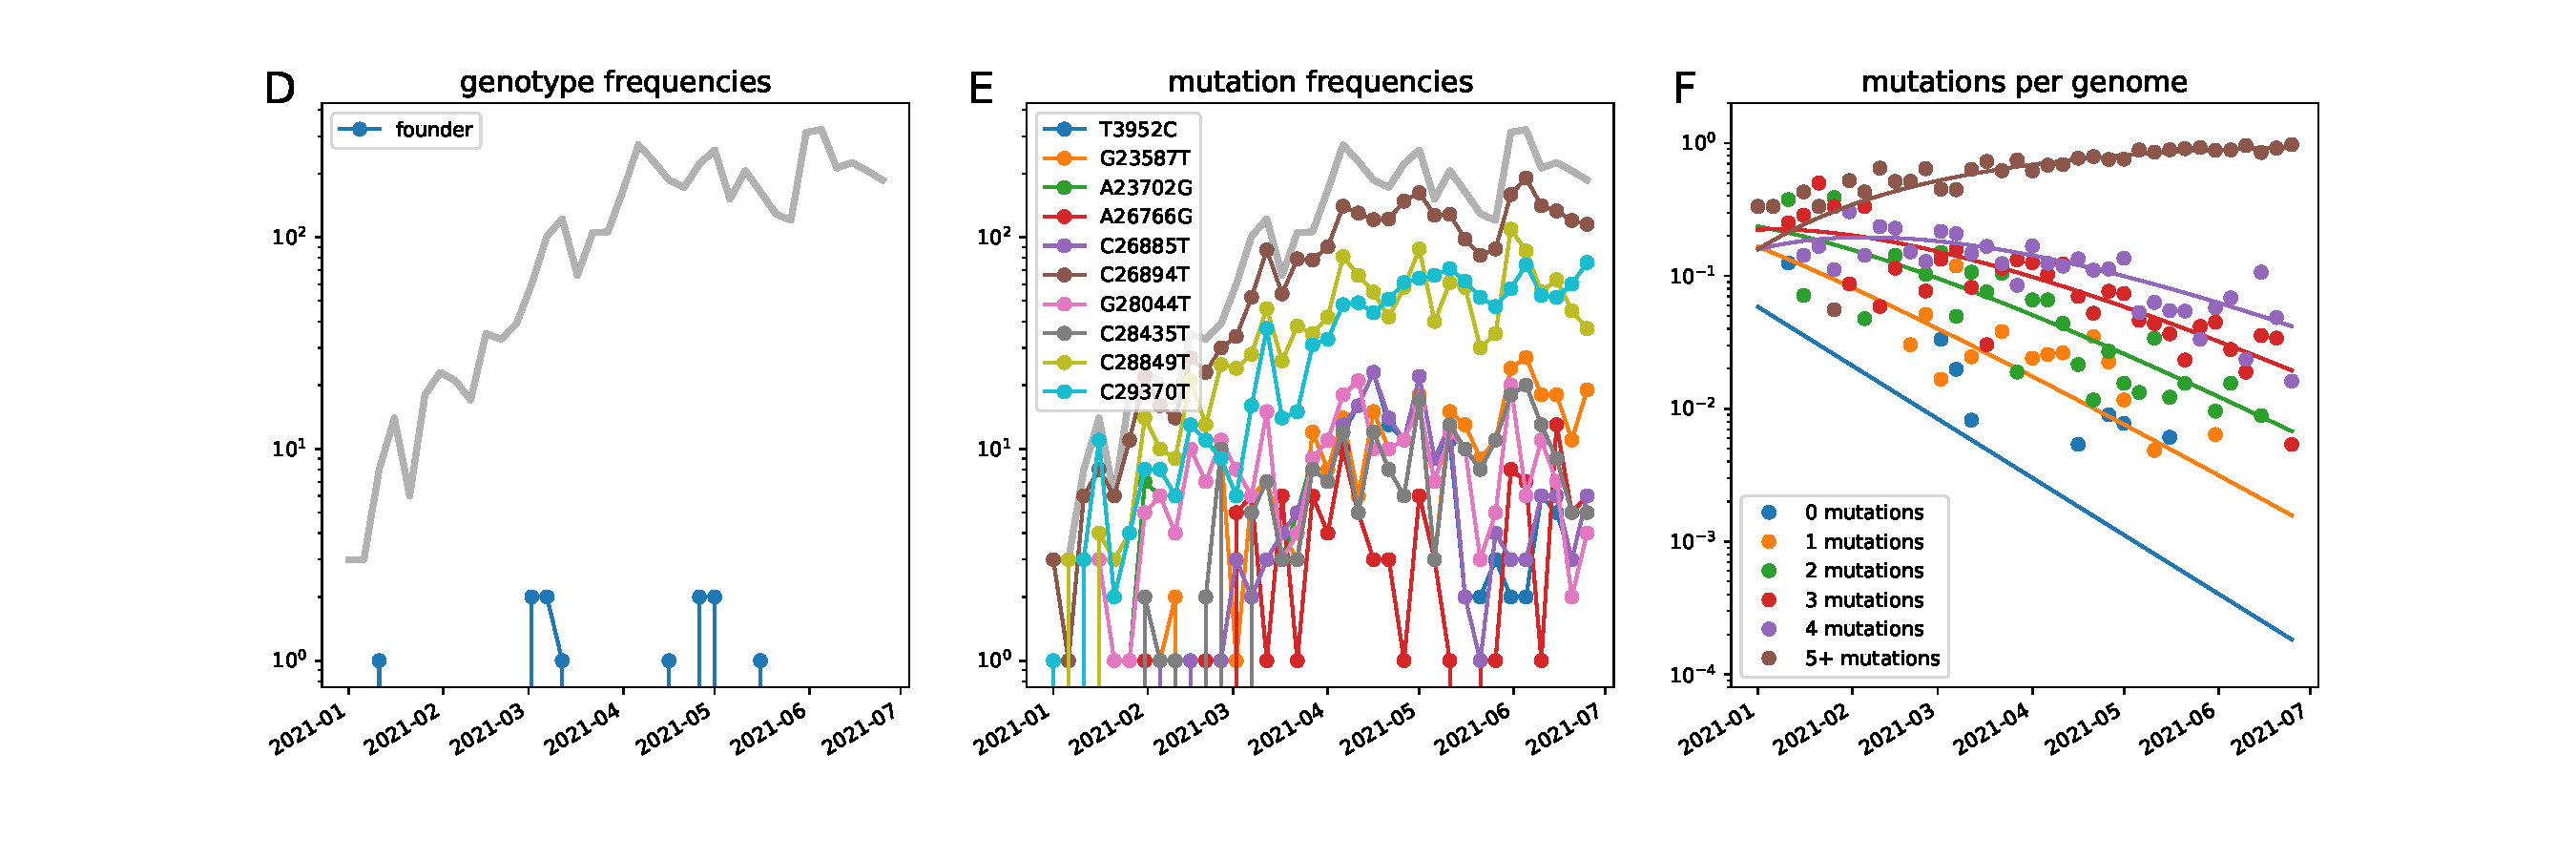
\includegraphics[width=\textwidth]{figures/counts/21G_counts.pdf}
    \caption{{\bf Diversification within clade 21G (Lambda).}
    \label{fig:21G_counts}}
\end{figure*}


\begin{figure*}[h]
    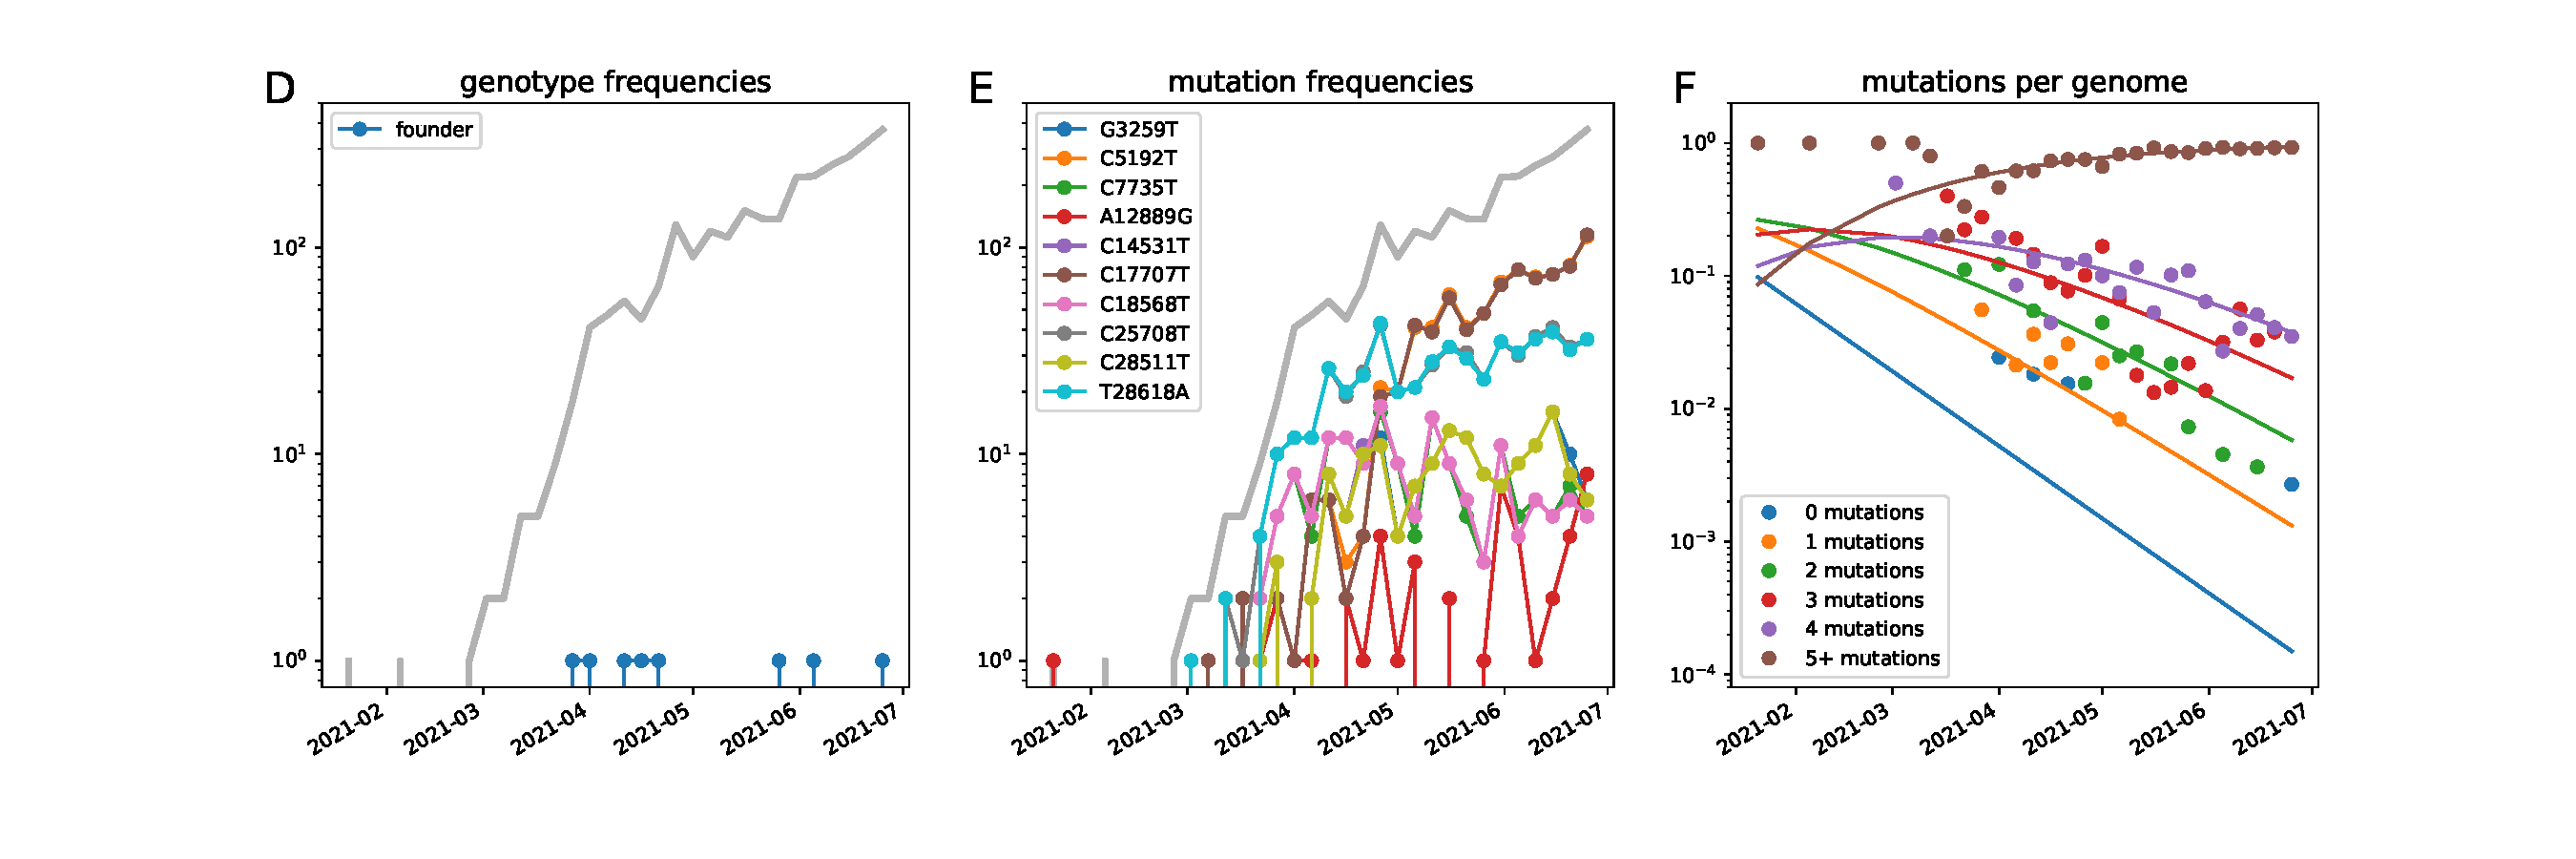
\includegraphics[width=\textwidth]{figures/counts/21H_counts.pdf}
    \caption{{\bf Diversification within clade 21H (Mu).}
    \label{fig:21H_counts}}
\end{figure*}



\begin{figure*}[h]
    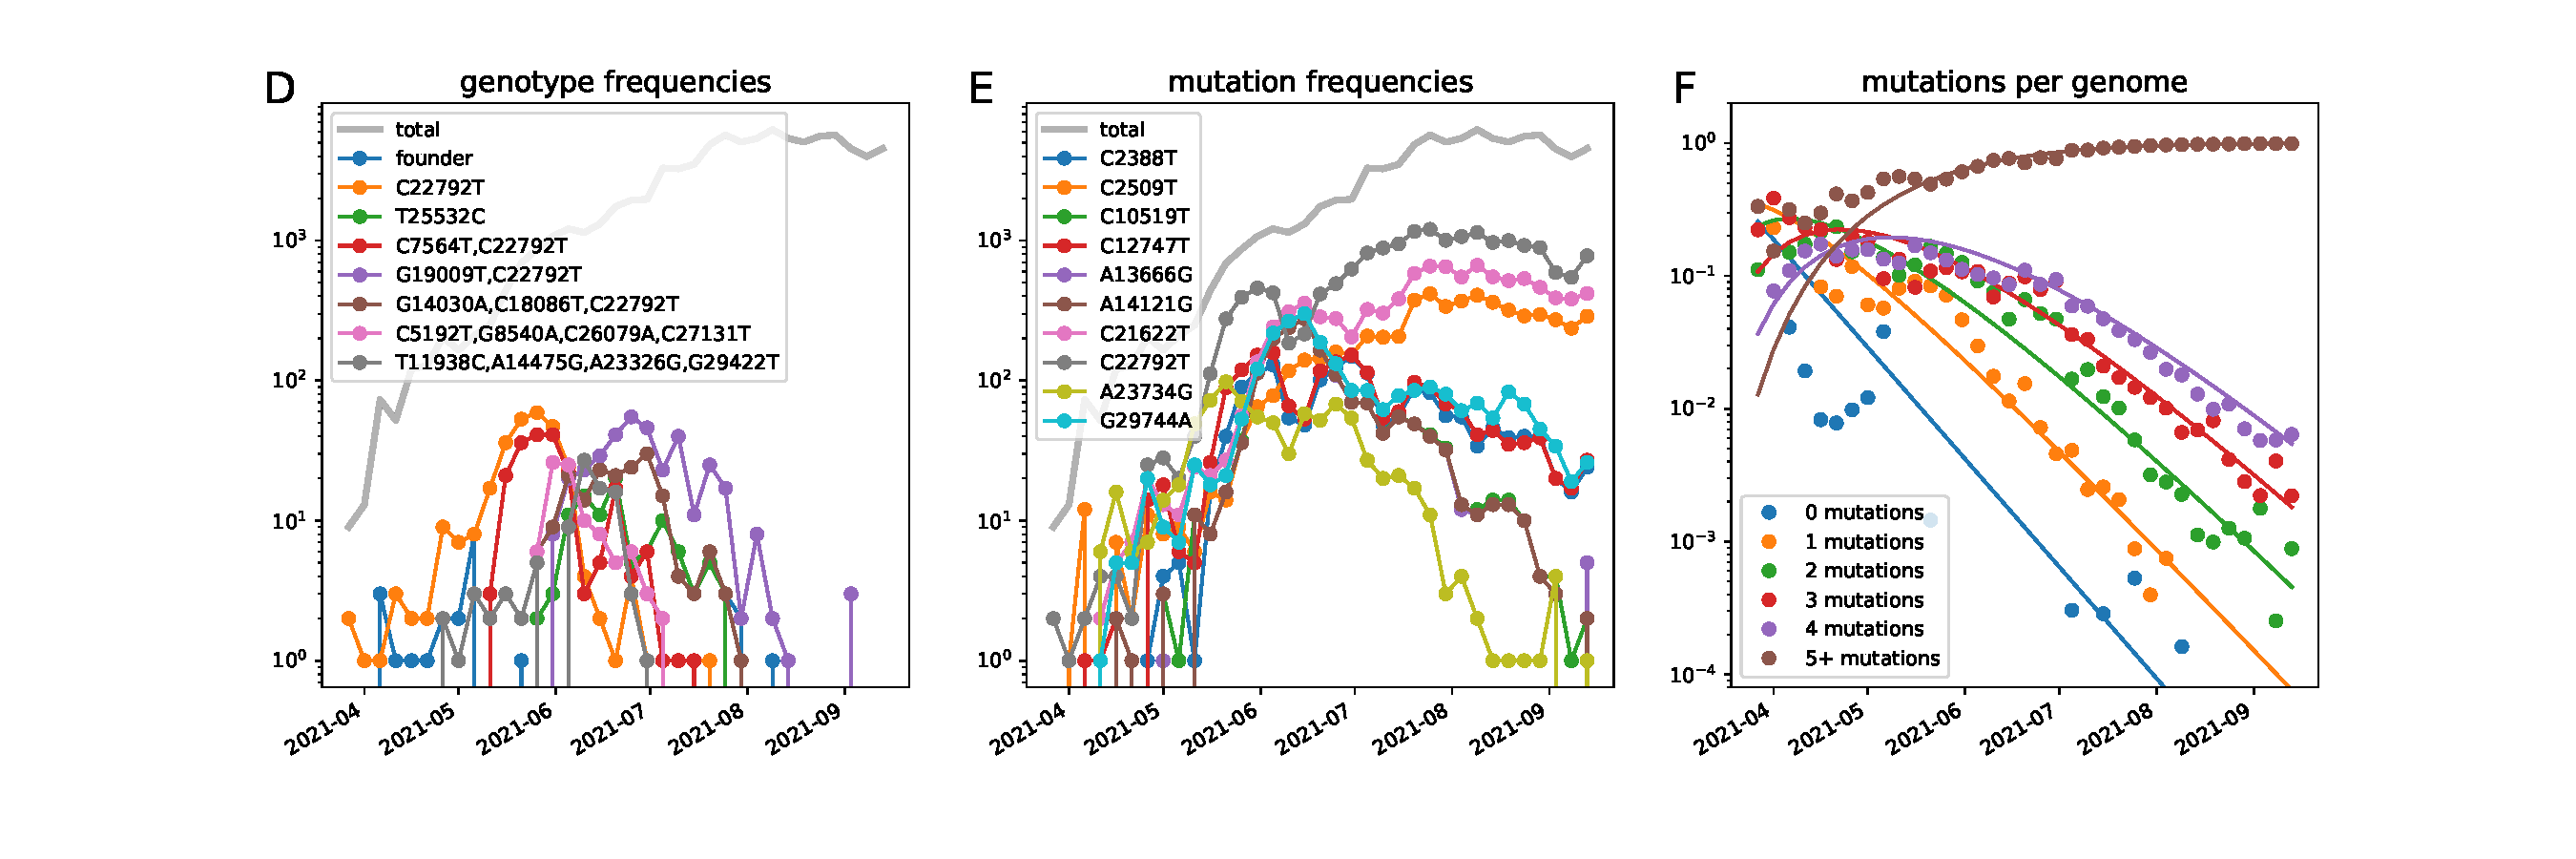
\includegraphics[width=\textwidth]{figures/counts/21I_counts.pdf}
    \caption{{\bf Diversification within clade 21I (Delta).}
    \label{fig:21I_counts}}
\end{figure*}


\begin{figure*}[h]
    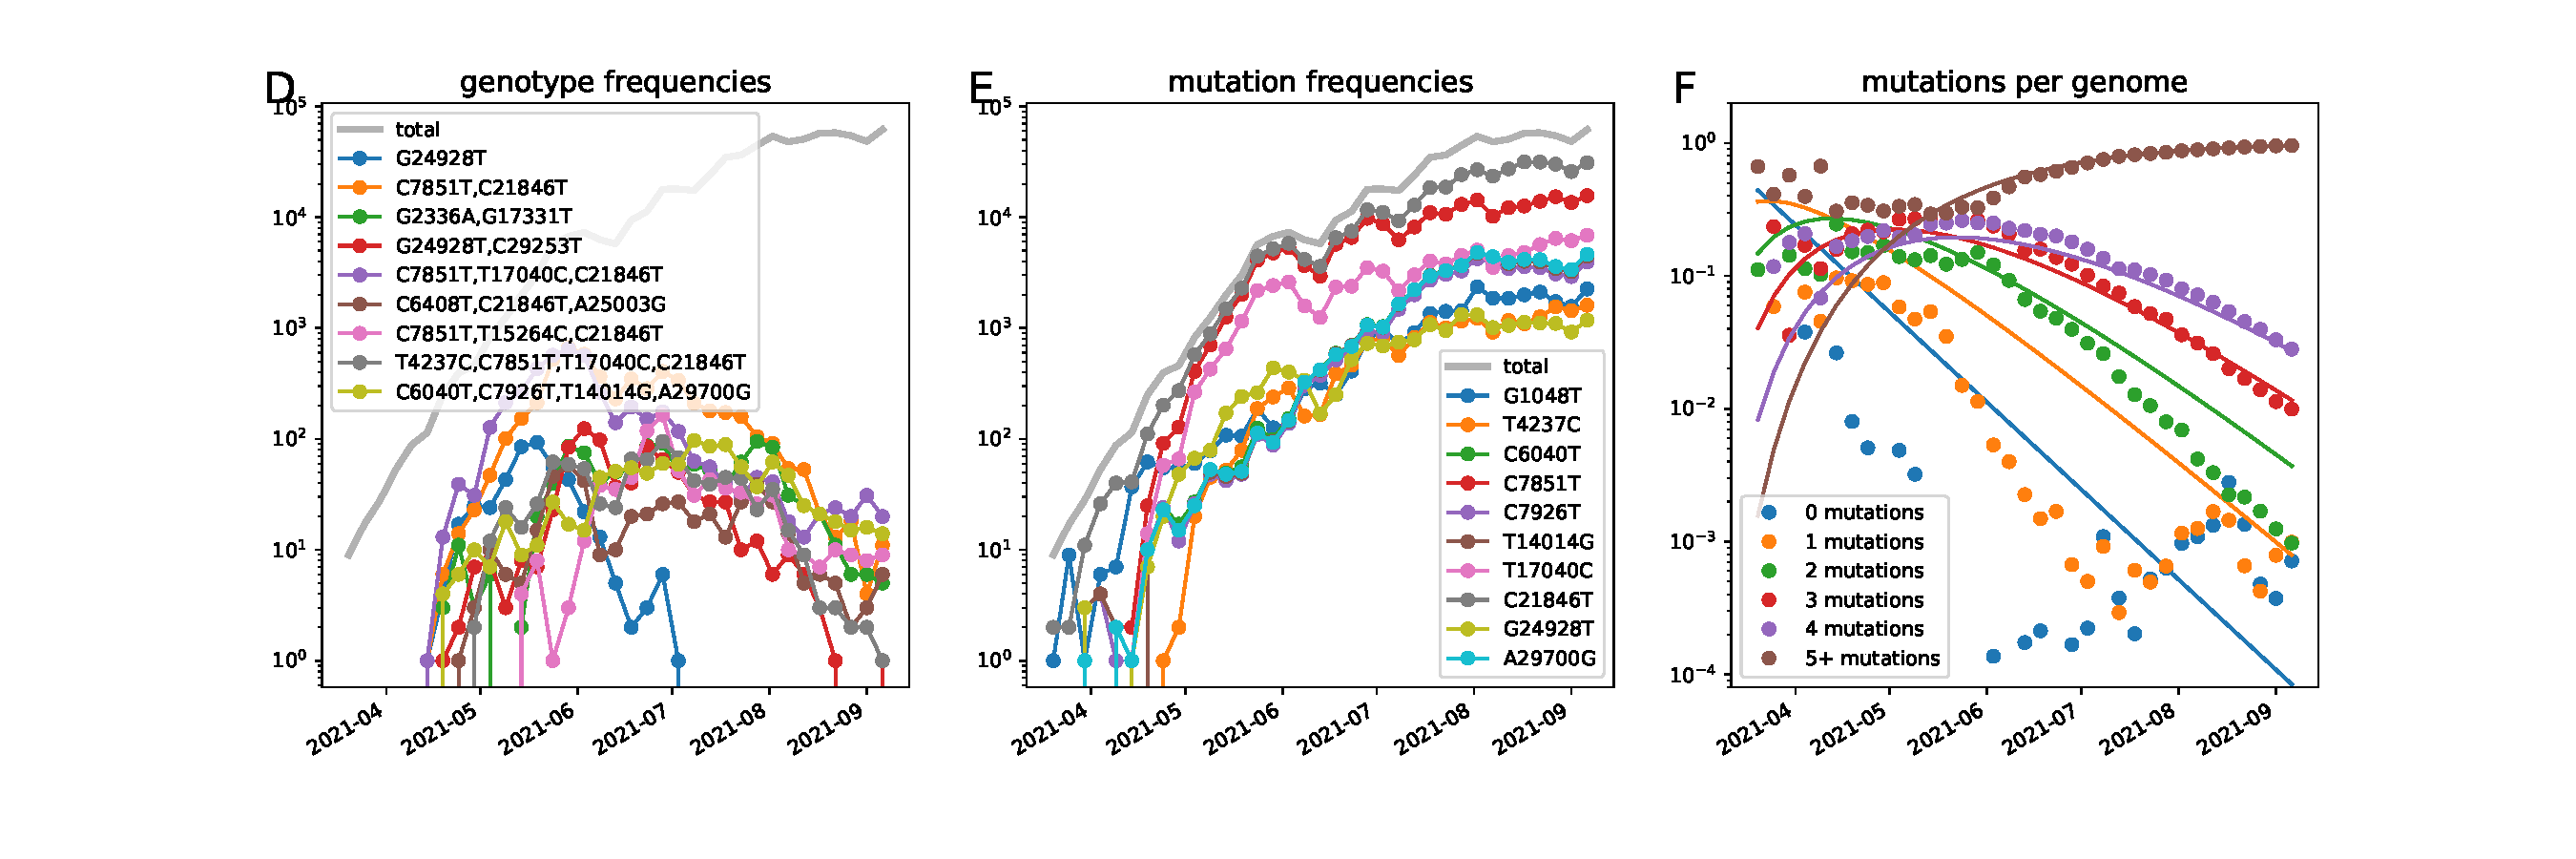
\includegraphics[width=\textwidth]{figures/counts/21J_counts.pdf}
    \caption{{\bf Diversification within clade 21J (Delta).}
    \label{fig:21J_counts}}
\end{figure*}

\begin{figure*}[h]
    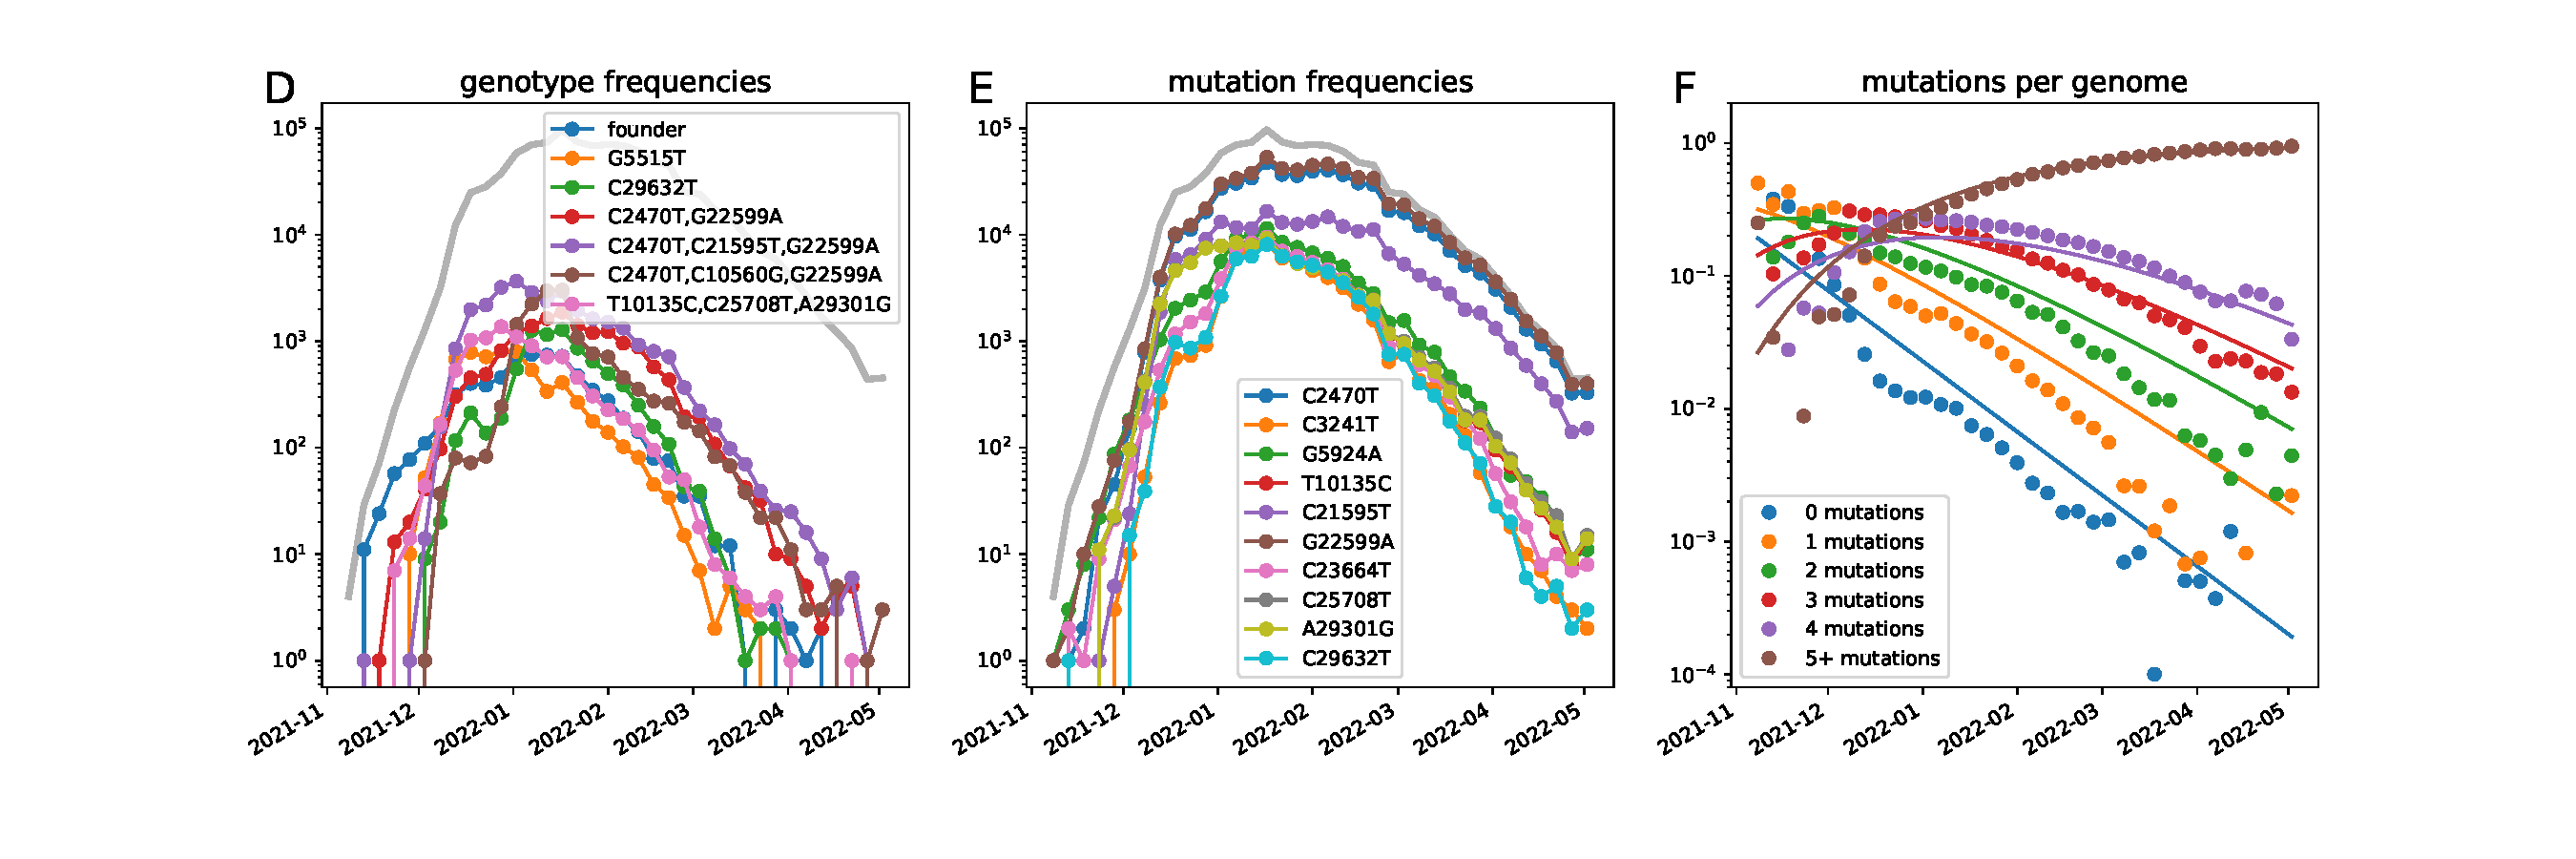
\includegraphics[width=\textwidth]{figures/counts/21K_counts.pdf}
    \caption{{\bf Diversification within clade 21K (Omicron).}
    \label{fig:21K_counts}}
\end{figure*}

\begin{figure*}[h]
    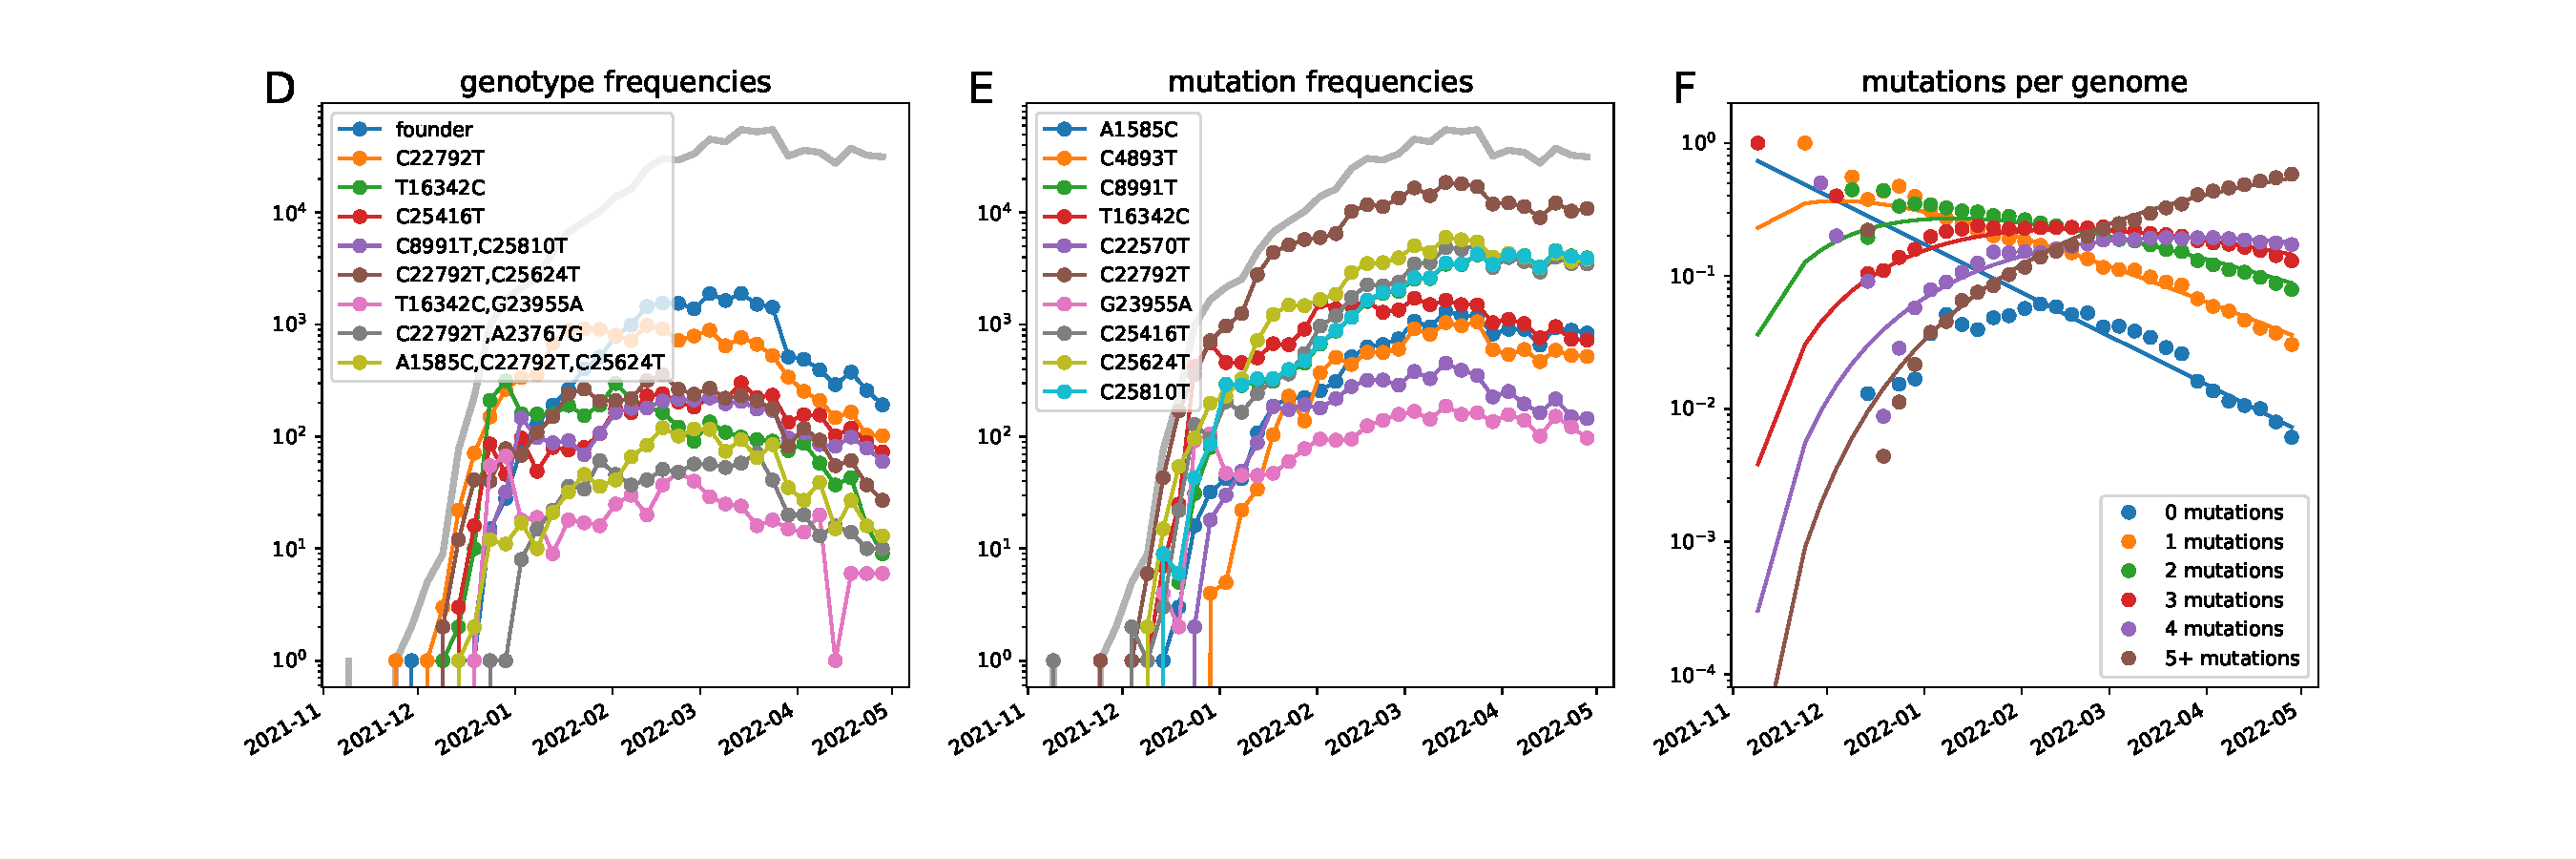
\includegraphics[width=\textwidth]{figures/counts/21L_counts.pdf}
    \caption{{\bf Diversification within clade 21L (Omicron).}
    \label{fig:21L_counts}}
\end{figure*}

\begin{figure*}[h]
    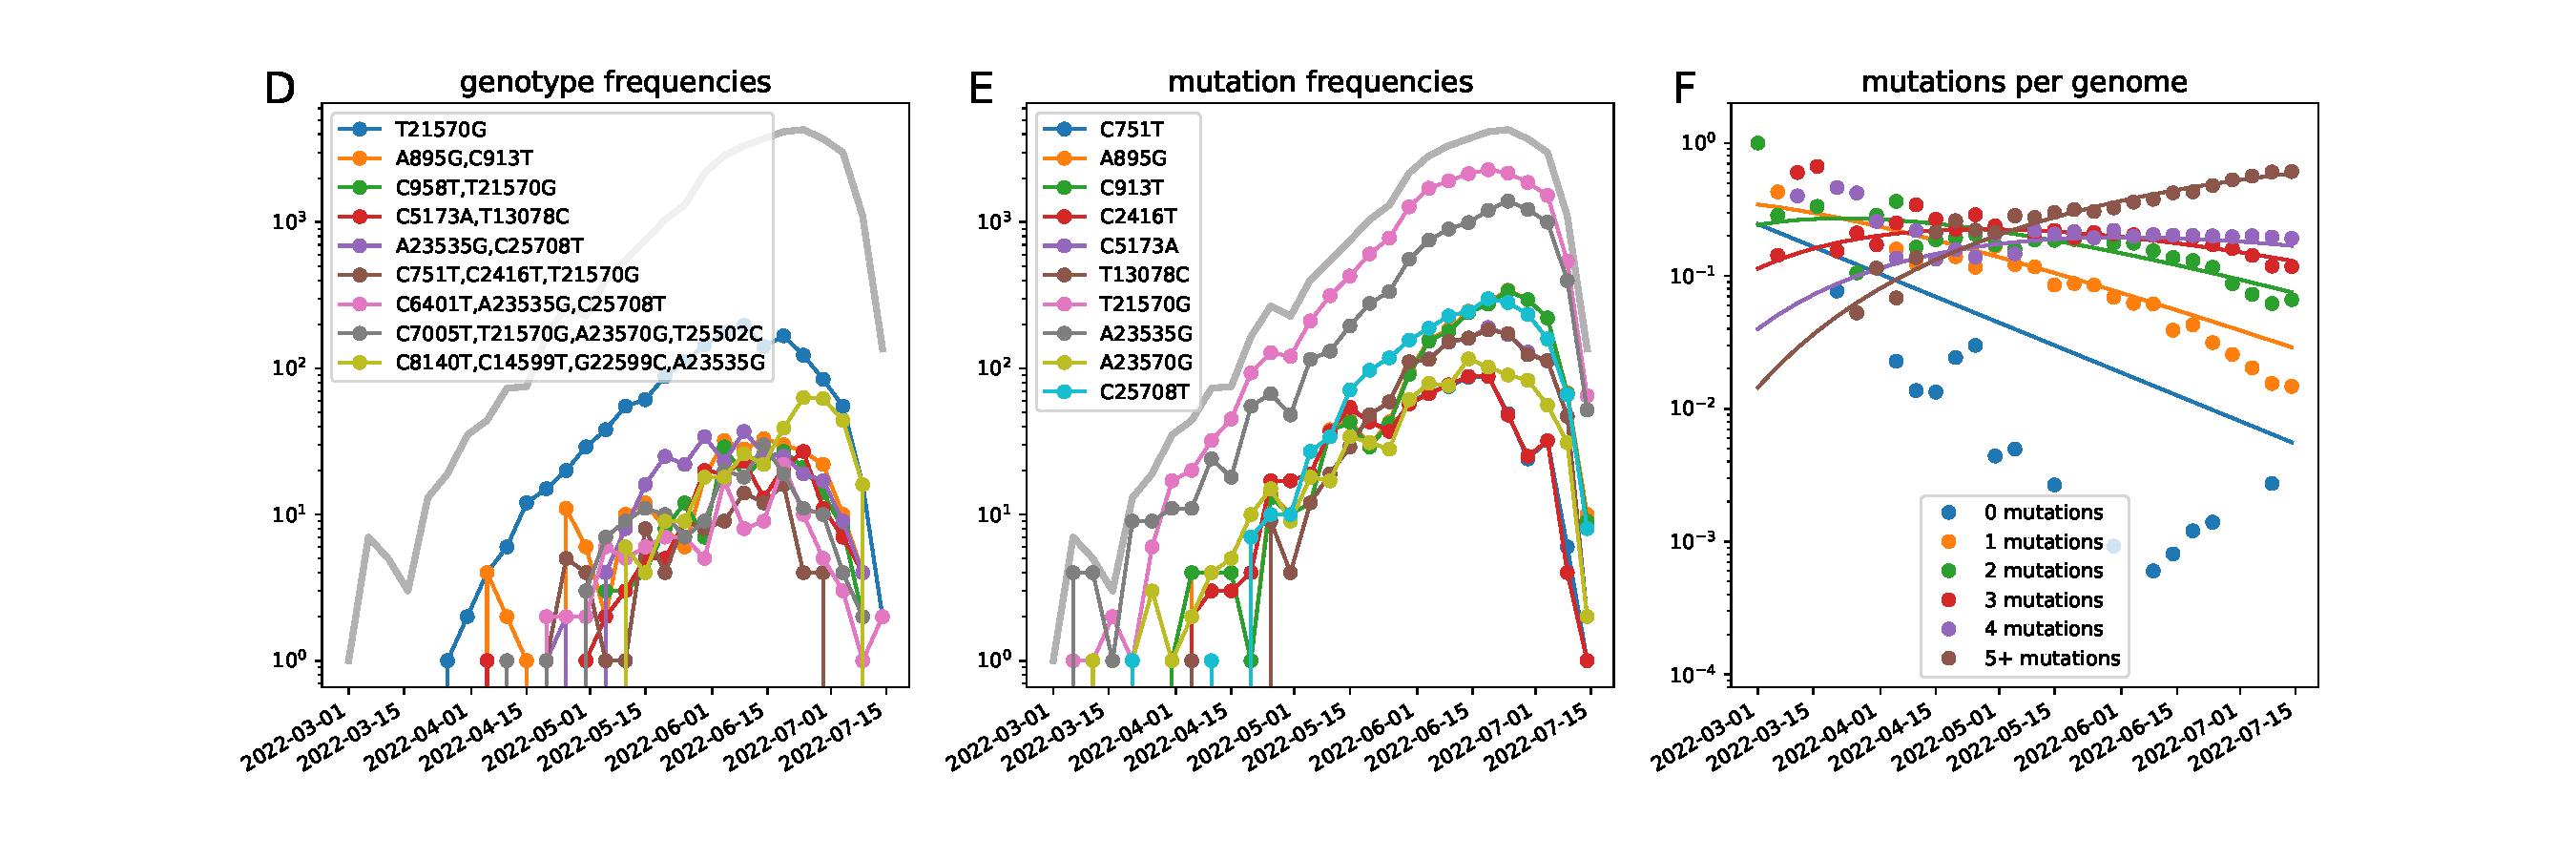
\includegraphics[width=\textwidth]{figures/counts/22A_counts.pdf}
    \caption{{\bf Diversification within clade 22A (Omicron).}
    \label{fig:22A_counts}}
\end{figure*}

\begin{figure*}[h]
    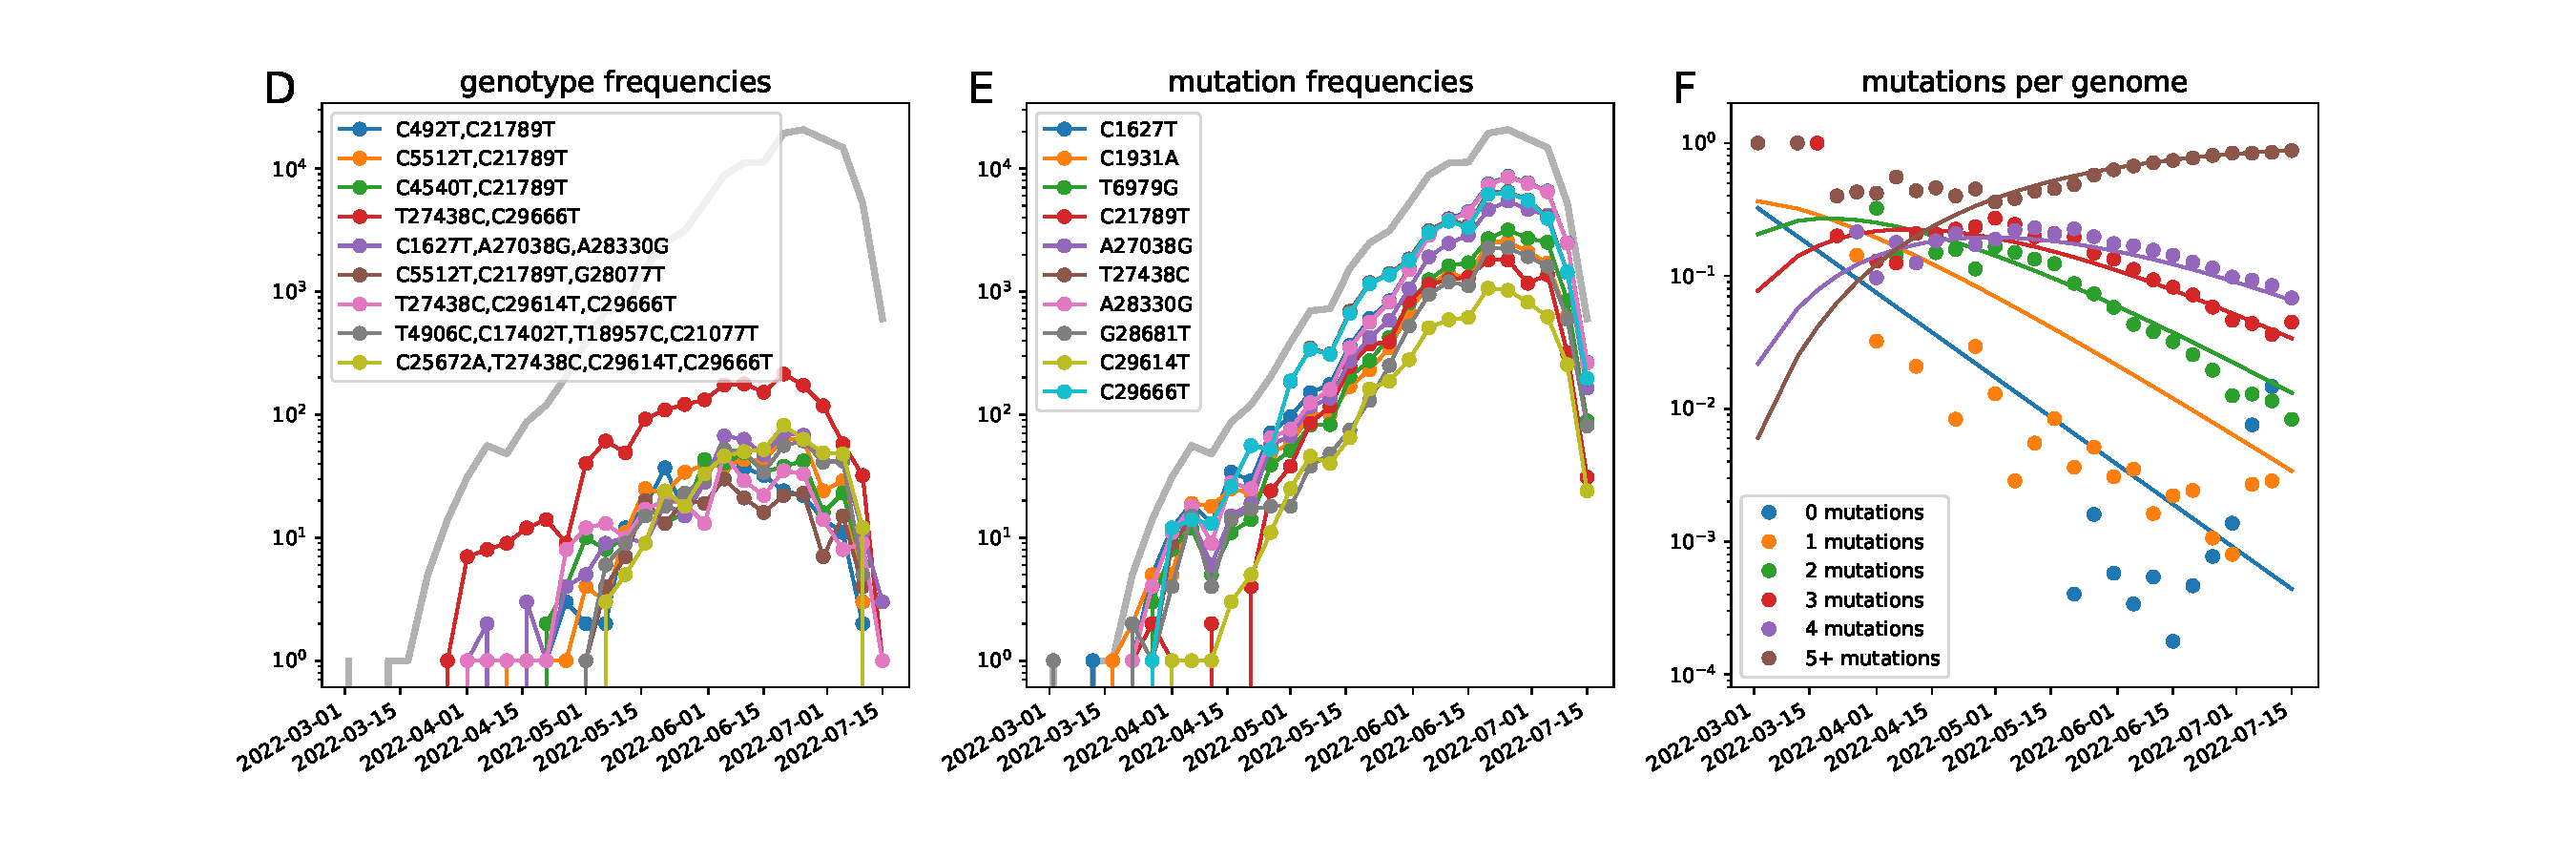
\includegraphics[width=\textwidth]{figures/counts/22B_counts.pdf}
    \caption{{\bf Diversification within clade 22B (Omicron).}
    \label{fig:22B_counts}}
\end{figure*}
